%% Thesis Template of Chinese Academy of Sciences
%%   for using CASthesis package with LaTeX2e
%%
%% Created by Ling-Yun Wu <aloft@ctex.org>
%%
%% $Id: template.tex,v 1.10 2007/01/09 05:10:46 aloft Exp $


%\documentclass[notypeinfo]{CASthesis}
\documentclass{CASthesis_zzk}
% 可选参数:
% notypeinfo 取消扉页的LaTeX版本信息
% dvips 使用 dvips 生成最终的 PS 文档


% 设置图形文件的搜索路径
\graphicspath{figures/}

% 取消链接的颜色(黑白打印时)
%\hypersetup{colorlinks=false}

% 小节标题靠左对齐
\CTEXsetup[format+={\flushleft}]{section}

%%%%%%%%%%%%%%%%%%%%%% BEGIN MY CONFIG %%%%%%%%%%%%%%%%%%%%%%
\input{fontsetup.tex}
% File Name: SetUp.tex
% Function: Make main settings of the document.


%%%%%%%%%%%%%%%%%%%%%%%%%%%%%% BEGIN-Packages %%%%%%%%%%%%%%%%%%%%%%%%%%%%%
\usepackage{amsmath,amsthm,amssymb,amsfonts}
\usepackage{mathrsfs}
\usepackage{graphicx}
\usepackage{enumerate}
\usepackage{booktabs}
\usepackage{tabularx}
\usepackage{multirow,multicol}
\usepackage{eqlist}
\usepackage{url}
\usepackage{cases}
\usepackage{subfigure} 
\usepackage{boxedminipage}
%\usepackage[section]{placeins}
\usepackage{placeins}
\usepackage{float}
\usepackage{longtable}
\usepackage{rotating}
\usepackage[ruled,lined,linesnumbered]{algorithm2e}
\usepackage{afterpage}  %在table和figure环境的标题中加脚注, footnotemark
\usepackage{changepage} %配合adjustwidth环境整体缩进

%\usepackage{titlesec}
%%%%%%%%%%%%%%%%%%%%%%%%%%%%%%%% END-Packages %%%%%%%%%%%%%%%%%%%%%%%%%%%%%


%%%%%%%%%%%%%%%%%%%% BEGIN-Theorem-like Environments %%%%%%%%%%%%%%%%%%%%%
\theoremstyle{plain}
%\newtheorem{Thm}{定理}[section]
\newtheorem{Thm}{\indent 定理}[chapter]
\newtheorem{Prop}[Thm]{\indent 命题}
\newtheorem{Lem}[Thm]{\indent 引理}
\newtheorem{Coro}[Thm]{\indent 推论}
\newtheorem{Rem}[Thm]{\indent 注}
\newtheorem{Asm}[Thm]{\indent 假设}
\newtheorem{Alg}[Thm]{\indent 算法}
\newtheorem{Cond}[Thm]{\indent 条件}
\newtheorem{Prob}[Thm]{\indent 问题}
\newtheorem{Def}[Thm]{\indent 定义}
\renewcommand{\proofname}{\indent {\heiti 证明}}
%\numberwithin{equation}{section}
\numberwithin{equation}{chapter}
%%%%%%%%%%%%%%%%%%%%% END-Theorem-like Environments %%%%%%%%%%%%%%%%%%%%%%

\graphicspath{{figures/}} % Set the directory where figures are saved.



%%%%%%%%%%%%%%%%%%%%%%%%%% BEGIN-New Commands %%%%%%%%%%%%%%%%%%%%%%%%%%%%
\newcommand{\chap}[1]{\textbf{Chapter} #1}

\newcommand{\ps}{\ \,}
\newcommand{\vect}{\textnormal{vec}}

\newcommand{\Gmf}{\Gamma\hskip-1mm}

\newcommand{\topcaption}{%
\setlength{\abovecaptionskip}{0pt}%
\setlength{\belowcaptionskip}{10pt}%
\caption}
\newcommand{\Bcaptionskip}{10pt}

\newcommand{\subfigwidth}{0.485\textwidth}
\newcommand{\namewidth}{1in}
\newcommand{\ski}{0.5em}
\newcommand{\comp}{\circ}
\newcommand{\hdp}{\!\comp\!}
\newcommand{\hdsq}[1]{#1^{\comp2}}
\newcommand{\hdsqrt}[1]{#1^{\comp\frac{1}{2}}}
\newcommand{\comps}{\!\comp\!}
\newcommand{\nxn}[0]{{n\times n}}
\newcommand{\dist}{\mathrm{dist}}
\newcommand{\diag}{\mathrm{diag}}
\newcommand{\pinv}[1]{#1^+}
%\newcommand{\pinv}[1]{#1^\dagger}
\newcommand{\tpinv}[1]{#1^{\dagger\textnormal{T}}}
\newcommand{\hpinv}[1]{#1^{\frac{1}{2}\dagger}}
\newcommand{\iti}[1]{\textnormal{(#1.)}}

\renewcommand{\baselinestretch}{1.3}
\renewcommand{\qedsymbol}{$\blacksquare$}
\renewcommand{\theenumi}{\textnormal{\alph{enumi}.)}}
\renewcommand{\labelenumi}{\theenumi}

\DeclareMathAlphabet{\mathcal}{OMS}{cmsy}{m}{n}    % Use standard calligrafic font of mathcal, instead of the rsfs one.
\newcommand{\fsp}[1]{\mathcal{#1}}       % Use mathcal font for function spaces.
\newcommand{\Qfs}{\fsp{Q}}      
\newcommand{\solver}{\mathcal{S}}
\newcommand{\prob}{\mathcal{P}}
%%%%%%%%%%%%%%%%%%%%%%%%%%%%%%%%%
\newcommand{\funl}[1]{\mathscr{#1}}      % Use Euler mathscr font for functionals.
\newcommand{\Fun}{\funl{F}}     
%%%%%%%%%%%%%%%%%%%%%%%%%%%%%%%%%
\DeclareMathAlphabet{\mathpzc}{OT1}{pzc}{m}{it}   
%\newcommand{\setrn}[1]{\mathpzc{#1}}     % Use mathpzc font for subsets of R^n.
\newcommand{\setrn}[1]{\mathcal{#1}}     % Use mathpzc font for subsets of R^n.
\newcommand{\set}{\setrn}
\newcommand{\Space}{\setrn}
\newcommand{\ball}{\setrn{B}}
\newcommand{\IntS}{\setrn{I}}
%%%%%%%%%%%%%%%%%%%%%%%%%%%%%%%%%
\newcommand{\kaibox}[1]{\mbox{\kaishu #1}}
\newcommand{\alg}[1]{\mbox{\textnormal{\texttt{#1}\ }}}      % Use \texttt for algrithm/software names.
\newcommand{\dfo}{\alg{DFO}}
\newcommand{\newuoa}{\alg{NEWUOA}}
\newcommand{\lfn}{\alg{LFN}}
\newcommand{\newuoam}{\alg{NEWUOAm}}
\newcommand{\newuoas}{\alg{NEWUOAs}}
\newcommand{\uobyqa}{\alg{UOBYQA}}
\newcommand{\bobyqa}{\alg{BOBYQA}}
\newcommand{\mnh}{\alg{MNH}}
\newcommand{\mads}{\alg{MADS}}
\newcommand{\gps}{\alg{GPS}}
\newcommand{\apps}{\alg{APPSPACK}}
\newcommand{\appspack}{\alg{APPSPACK}}
\newcommand{\nmsmax}{\alg{NMSMAX}}
\newcommand{\imfil}{\alg{IMFIL}}
\newcommand{\condor}{\alg{CONDOR}}
\newcommand{\cobyla}{\alg{COBYLA}}
\newcommand{\orbit}{\alg{ORBIT}}
\newcommand{\dfls}{\alg{DFLS}}
\newcommand{\boosters}{\alg{BOOSTERS}}
\newcommand{\SYMB}{\alg{SYMB}}
\newcommand{\ESYMBS}{\alg{ESYMBS}}
\newcommand{\ESYMBP}{\alg{ESYMBP}}
\newcommand{\fmins}{\alg{fminsearch}}
\newcommand{\lancelot}{\alg{LANCELOT}}
\newcommand{\subi}{\alg{SUBSPACE1}}
\newcommand{\subii}{\alg{SUBSPACE2}}
\newcommand{\subiii}{\alg{SUBSPACE3}}
\newcommand{\subspace}{\alg{SUBSPACE}}
\newcommand{\psub}{\alg{PSUB}}
\newcommand{\cuter}{\alg{CUTEr}}
\newcommand{\matlab}{\textsc{Matlab}\ }  % Use \textsc for Matlab.
\newcommand{\subrout}[2]{\textnormal{\texttt{#1}}\textnormal{(}#2\textnormal{)}}
%%%%%%%%%%%%%%%%%%%%%%%%%%%%%%%%%
\newcommand{\Real}{\mathbb{R}}
\newcommand{\Complex}{\mathbb{C}}
\renewcommand{\Re}{\mathrm{Re}}
\renewcommand{\Im}{\mathrm{Im}}
\newcommand{\Tran}[1]{#1^\mathrm{T}}
\newcommand{\tF}{\textnormal{F}}
\newcommand{\st}{\textnormal{s.t.}}
\newcommand{\Tr}{\mathrm{Tr}}
\newcommand{\Span}{\mathrm{span}}
\newcommand{\sign}{\mathrm{sign}}
\newcommand{\ran}{\mathcal{R}}
%\newcommand{\Sob}[2]{W_#1^#2}
\newcommand{\Sob}[2]{{H^#2}}
\newcommand{\SobH}[2]{{H^{#2,#1}}}
%%%%%%%%%%%%%%%%%%%%%%%%%%%%%%%%%%
\newcommand{\md}{\,\mathrm{d}}
\newcommand{\me}{\mathrm{e}}
\newcommand{\betaf}{\beta\!}
\newcommand{\Gammaf}{\Gamma\!}
\newcommand{\ellp}{\ell_p}
\newcommand{\ellt}{\ell_2}
\newcommand{\ello}{\ell_1}
\newcommand{\elli}{\ell_\infty}
\newcommand{\radius}{r}
\newcommand{\mean}{\mathrm{mean}}
\newcommand{\std}{\mathrm{std}}
\newcommand{\rstd}{\mathrm{rstd}}


%%%%%%%%%%%%%%%%%%%%%%%%%%%%%%%%%%%%%%%%%%%
% szl thesis
\newcommand{\xn}{x_1,x_2,\ldots,x_n} 
\newcommand{\be}{\begin{equation}}
\newcommand{\ee}{\end{equation}}
\newcommand{\ba}{\begin{array}}
\newcommand{\ea}{\end{array}}
\newcommand{\bc}{\begin{center}}
\newcommand{\ec}{\end{center}}
\newcommand{\bl}{\begin{flushleft}}
\newcommand{\el}{\end{flushleft}}
%\newcommand{\pozhe}{\raisebox{0.5mm}{------}}
\newcommand{\pozhe}{---\hspace*{-2mm}---} %中文破折号
\newcommand{\hd}[1]{\multicolumn{1}{c}{#1}}
%%%%%%%%%%%%%%%%%%%%%%%%%%%%%%%%%%%%%%%%%%%


\def\mathllap{\mathpalette\mathllapinternal}
\def\mathllapinternal#1#2{%
\llap{$\mathsurround=0pt#1{#2}$}%
}
\def\clap#1{\hbox to 0pt{\hss#1\hss}}
\def\mathclap{\mathpalette\mathclapinternal}
\def\mathclapinternal#1#2{%
\clap{$\mathsurround=0pt#1{#2}$}%
}
\def\mathrlap{\mathpalette\mathrlapinternal}
\def\mathrlapinternal#1#2{%
\rlap{$\mathsurround=0pt#1{#2}$}%
}


%%%%%%%%%%%%%%%%%%%%%%%%%%%%END-NewCommands%%%%%%%%%%%%%%%%%%%%%%%%%%%%

\renewcommand\thesection{\S\,\arabic{chapter}.\arabic{section}}
\usepackage{makeidx,tocbibind}
\makeindex
%%%%%%%%%%%%%%%%%%%%%% END MY CONFIG %%%%%%%%%%%%%%%%%%%%%%
  
\begin{document}

%%%%%%%%%%%%%%%%%%%%%%%%%%%%%%
%% 封面部分
%%%%%%%%%%%%%%%%%%%%%%%%%%%%%%
  
  % 中文封面内容
  \classification{}
  \confidential{}
  \UDC{}
  \serialnumber{}
  \title{距离几何问题的理论及应用}
  \author{盛镇醴}
  \advisor{袁亚湘 (院士、研究员、博士)}
  \advisorinstitute{中国科学院数学与系统科学研究院}
  \degree{博士}
  \degreetype{理学博士}
  \major{计算数学}
  \submitdate{2015年4月}
  \defenddate{2015年5月}
  \institute{中国科学院数学与系统科学研究院}
%  \school{中国科学院研究生院}
%\school{\includegraphics[width=0.9\textwidth]{GUCAS.pdf}}
%\school{\includegraphics[width=0.9\textwidth]{gucas-zzk.eps}}
  \chairman{}
  
  % 英文封面内容
  \englishtitle{Distance Geometry Problem: Theory and Applications}
  \englishauthor{Zhenli Sheng}
  \englishadvisor{Prof. Ya-Xiang Yuan}
  \englishinstitute{Institute of Computational Mathematics and Scientific/Engineering
  Computing\\
    Academy of Mathematics and Systems Science \\
    Chinese Academy of Sciences}
  \englishdegree{Ph.D.}
  \englishmajor{Computational Mathematics}
  \englishdate{April, 2015}


  % 封面
  \pdfbookmark[0]{封面}{titlepage}
  \renewcommand{\thepage}{\alph{page}}
  \maketitle
  % 英文封面
  \makeenglishtitle
  

%%%%%%%%%%%%%%%%%%%%%%%%%%%%%%
%% 前言部分
%%%%%%%%%%%%%%%%%%%%%%%%%%%%%%
\frontmatter
\cleardoublepage
\thispagestyle{empty}
{\begin{center}
%    {\Huge{\kaishu 献给我的父亲母亲}}
    {\Huge{\xingkai 献给我的父亲母亲}}
%    {\Huge{\xinwei 献给我的父亲母亲}}
\end{center}
}
\newpage
\thispagestyle{empty}
The subject of optimization is a fascinating blend of heuristics and rigour,
of theory and experiment.
\begin{flushright}
    --- R. Fletcher, \emph{Practical Methods of Optimization}
\end{flushright}

\vskip1em
In fact, we consider optimization without derivatives one of the most important, open,
and challenging areas in computational science and engineering, and one with
enormous practical potential. 
\begin{flushright}
    --- A. R. Conn, K. Scheinberg, and L. N. Vicente,\\ \emph{Introduction to Derivative-Free Optimization}
\end{flushright}


\setcounter{page}{0}
  % 摘要
  
 \begin{abstract}

因为其广泛的应用, 距离几何问题 (Distance Geometry Problem)
在最近几十年成为了一个跨学科的研究热点. 
本文就是围绕这一问题, 针对其建模, 算法分析及设计进行了研究.

距离几何问题通常都建模成一个优化问题来求解, 
但不同的文献提出了多个误差函数建模成不同的问题, 
本文首先综述了各文献中使用的误差函数, 分析其优劣, 
并在此基础上提出了我们自己的误差函数.

文章综述了已有的一些算法,
尤其是针对一类半定规划 (Semidefinite Programming, 简称SDP) 算法, 
和一类几何构建 (Geometric Buildup, 简称GB) 算法,
我们比较了算法求解的问题形式, 求解速度和精度.

基于原有的几何构建算法, 我们提出改进的带误差函数优化的几何构建算法
(enhanced Geometric Buildup algorithm with Error Minimization, 简称GBEM).
新的算法主要有两方面的改进: 首先, 我们分析并用小例子展示了计算顺序对
算法结果的重要影响, 我们提出了新的规则谨慎选择每次加入的点, 
数值实验表明, 新的算法较原有算法, 稳定性大幅提高. 其次, 我们提出了一个
新的算法框架, 将误差函数优化整合进了原有算法, 进而有效地控制了误差累积的问题,
这是原有算法最大的缺陷. 深入的数值实验表明, 新的算法能在相对短的计算时间内,
得到合理精确的数值结果. 例如, 给定原子间小于 6\AA 的全部距离, 但是随机
添加不大于 10\% 的乘性噪音, 一个有 5681 个原子的蛋白质能够在3分钟之内被
定位, 得到的最小均方误差 (Root Mean Squared Deviation, 简称RMSD) 为0.24\AA.
已有的最新的几个构建算法在给定距离小于 6\AA 的情况下最多只能处理0.01\%的噪音, 
我们的新算法可以处理10\%的误差, 这使得新的算法能够真正用来解决实际问题.
这是本文得到的最有效的算法.

除此之外, 我们还研究了针对该问题的分布式算法. 
分布式算法是求解大规模问题的常用手段, 
但该问题有其特殊性, 因为我们已知的只有局部点之间的距离信息,
缺乏有效的空间信息, 如何有效地分割原问题是一大难点.
我们将距离几何问题看作一个图上的问题, 研究图的拉普拉斯(Laplace)矩阵,
基于其特征向量映射将原问题分割成一些可以高效求解的小规模问题.
初步的数值实验结果表明, 这种新的思路是有效的.





大多数优化方法都依赖问题的导数信息.\ps 但是,\ps 在实际应用中,\ps 大量问题的
导数信息都是不可用的.\ps 这就要求我们研究不使用导数信息的方法,\ps 这就是
本文研究的无导数优化算法.\ps 

算法的评价是算法研究中的重要问题.\ps 
我们研究了如何客观可信地评价和比较不同的无导数优化算法.\ps 
我们用一个例子清楚地说明传统的评价方法对于无导数算法是不可靠的.\ps 
通过引入统计的方法,\ps 我们建立了评价无导数方法的一套新体系.
与传统的评价方法相比,\ps 新方法不但能够
反映算法对计算机舍入误差的稳定性,\ps 而且能更可靠的度量
算法的计算开销.\ps 

%第\ref{chap:lfn}章研究了无导数优化算法中的
最小 Frobenius 范数插值和对称 Broyden 修正是无导数信赖域方法中最有效
的两种建立模型的方式.\ps 
我们第一次指出了这两种方式在一些情况下的等价性.\ps 
与这两种模型紧密相关的一个问题是 \newuoa 算法的重开始技术.\ps 
通过修改 \newuoa 源代码中的重开始条件,\ps 我们给出了一个改进版本的
\newuoa 代码.\ps 新版代码仅仅删除了原始代码中的四个字母,\ps 就显著
降低了代码的计算开销,\ps 并且明显提高了代码对计算机舍入误差的稳定性.\ps 
我们系统地比较了最小 Frobenius 范数模型和对称 Broyden 修正在 \newuoa 算法
框架下的表现,\ps 并且指出,\ps  
当求解精度不太高时,\ps 
最小 Frobenius 范数模型比对称 Broyden 修正建立的模型表现更好.\ps 
这一事实对于实际应用领域很有意义,\ps
因为实际的无导数优化问题对解的精度要求往往不高.\ps 

为了研究无导数优化中有广泛应用的最小范数插值,\ps
我们率先将 PDE 理论中的 Sobolev 范数和半范数
引入无导数算法的研究中.\ps 我们用二次函数的系数
给出了二次函数在 $\ellp$ 球上的 $\Sob{2}{0}$
范数和 $\Sob{2}{1}$ 半范数的显式表达式.\ps 
我们证明,\ps 最小
范数插值实际上是在一个 $\ellt$ 球上极小化插值函数的 $\Sob{2}{1}$ 半范数.\ps 
这一观察为理解最小范数插值提供了有力的工具.\ps 
通过这一观察,\ps 我们首次指出了最小范数插值中两个参量的几何意义.\ps 
我们将这些理论用于研究扩展的对称 Broyden 修正,\ps 
得到了简单并且有效的参数选取方式.\ps 

到目前为止,\ps 无导数方法可求解的问题规模还十分有限.\ps 为了求解大规模问题,\ps 
我们提出了两种无导数的子空间算法.\ps 
在第一种子空间方法中,\ps 利用 Hooke-Jeeves
模式搜索的思想,\ps 针对无导数信赖域方法,\ps
我们提出在子空间上求解信赖域子问题的策略.\ps
这种子空间策略改善了 \newuoa 算法的数值表现.
第二种子空间方法,\ps 即 
\newuoas (A \texttt{NEW} \texttt{U}nconstrained \texttt{O}ptimization 
\texttt{A}lgorithm with \texttt{s}ubspace technique based on \newuoa\!\!)
算法,\ps 是本文最大的亮点.\ps 其基本想法是,\ps 把一个大规模无导数优化问题
转化为一系列低维子问题.\ps 
我们首先研究了一个一般性的子空间算法框架,\ps 建立了其全局收敛性和 R-线性收敛速度.\ps 
然后,\ps 使用 \newuoa 算法作为子问题的求解器,\ps 我们不依赖导数地实现了该
框架,\ps 得到了 \newuoas 算法.\ps 
我们证明了 \newuoas 算法在理论上的全局收敛性、R-线性收敛速度和计算上的有限
终止性.\ps 我们还提出了一项预条件技术,\ps 显著改善了 \newuoas 算法对坏条件问题
的表现.\ps 据本文作者所知,\ps 这是无导数算法中第一次引入预条件技术.\ps 
实验证明,\ps \newuoas 算法不论在函数值计算次数、CPU 时间还是对计算机舍入误差的稳定性
上都明显
优于 \newuoa 算法,\ps 后者是目前最优秀的
无导数算法之一.\ps 我们还发现,\ps \newuoas 算法很适合求解初始点质量较差的问题,\ps 
这对实际应用领域很有意义,\ps 因为很多实际问题很难给出一个好的初始点.
不仅如此,\ps 对于很多维数高达 $2000$ 的测试问题, \newuoas 算法可以在几分钟内求
到精度很高的解,\ps 且使用的函数值计算次数不超过 $50000$ (相当于不到 25 个单纯形
梯度).
这是一个突破,\ps 因为
目前大部分无导数算法 (包括 \newuoa 算法) 至多可以求解几百维的问题;\ps 
对于它们,\ps $2000$ 维的问题几乎是不可求解的.

\keywords{无导数优化,\ps 信赖域方法,\ps 二次插值,\ps
对称 Broyden 修正,\ps Sobolev 半范数,\ps 子空间方法,\ps 大规模问题}
\end{abstract}


\begin{englishabstract}
Most of the optimization algorithms depend on derivative information of the
problem. However, there are numerous real-world 
problems where derivatives are unavailable. 
This motivates us to study derivative-free optimization methods.

The assessment and comparison of algorithms play important roles in the 
research of algorithms. We study how to assess derivative-free
algorithms in a reliable way. Through an example, we show that
it is not reliable to merely count the number of function evaluations. 
By introducing statistical method, we establish a new system for the 
assessment of derivative-free algorithms.   
The new system reflects the stability of algorithms with respect to 
computer rounding errors, and provides more convincing comparison of 
different algorithms.

Least Frobenius norm quadratic interpolation and symmetric Broyden update are the most 
successful methods of constructing models in derivative-free trust-region
algorithms. We prove the equivalence between these 
two strategies in some cases. The restart technique in \newuoa is closely 
related to these two strategies. We modify the restart criterion in the
source code of \newuoa by simply deleting four letters and obtain a 
new version of the source code.
The modification brings considerable improvement. Under the framework of \newuoa\!\!,
we compare 
least Frobenius norm model and the 
model established by symmetric Broyden update. We point out that 
least Frobenius norm model works better if a low-precision minimizer 
is desirable, 
which is meaningful for applications, because many 
problems in practice do not require high-precision
solutions.

To study the widely-used least norm quadratic interpolation in derivative-free
methods, we introduce the Sobolev norms and seminorms, which are classical
in PDE theory but rarely noticed in optimization.
For the $\Sob{2}{0}$ norm and $\Sob{2}{1}$
seminorm of a quadratic function over an $\ellp$ ball,  
we obtain explicit formulae in terms of the coefficients of the 
function.
We prove that least norm quadratic interpolation seeks an interpolant
with minimal $\Sob{2}{1}$ seminorm over an $\ellt$ ball.
This observation provides a new perspective to interpret the interpolation.
Consequently, we present the geometrical meaning of 
the parameters in the interpolation. We apply our theory to 
study the extended symmetric Broyden update, and propose a very simple but
effective way of choosing the parameters in the update. 

Until now, derivative-free methods can only solve problems with modest dimension.
We study subspace techniques to attack large scale problems. 
We presents two derivative-free subspace methods.
In the first method, we apply the idea of Hooke-Jeeves pattern-search to
derivative-free trust-region method, and propose to solve the trust-region
subproblem in a low-dimensional subspace of $\Real^n$.
This subspace strategy 
improves the performance of \newuoa\!\!. The second subspace method, which
is named as \newuoas\!\!, 
%(A \texttt{NEW} \texttt{U}nconstrained \texttt{O}ptimization 
%\texttt{A}lgorithm with \texttt{s}ubspace technique based on \newuoa\!\!),
is the highlight of the thesis. Its basic idea is to
divide a large scale problem into a sequence of low-dimensional subproblems.
We first study a general subspace
algorithm based on this idea, and present its convergence theory.
Then using \newuoa as the subproblem solver,
we implement the algorithm without using derivatives and obtain \newuoas\!\!.
For \newuoas\!\!, we establish its global convergence and R-linear convergence rate
in theory, and prove its finite termination in computation. We propose a 
preconditioning technique, which improves the performance of \newuoas on
ill-conditioned problems. As far as we know, this is the first derivative-free
algorithm with preconditioning procedure. In our numerical experiments,
\newuoas works evidently better than \newuoa\!\!, in the number of function evaluations,
CPU time, and stability.\ps 
We also find that \newuoas is good at solving problems with bad starting points,
which is favourable in real-world applications. Besides, 
\newuoas is capable of solving many $2000$-dimensional test problems to high precision 
within several minutes, using not more than $50000$ function evaluations
(equivalent to less than 25 simplex gradients).
It is a breakthrough, because most state-of-the-art derivative-free algorithms
can only solve problems with not more than a few hundreds of variables,
and $2000$-dimensional problems are nearly unsolvable for them.

\englishkeywords{derivative-free optimization, trust-region method, 
quadratic interpolation, symmetric Broyden update, Sobolev seminorm,
subspace method, large scale problem}
\end{englishabstract}


  % 目录
  \tableofcontents
  % 表格目录
  \listoftables
  % 插图目录
  \listoffigures
%
%
%%%%%%%%%%%%%%%%%%%%%%%%%%%%%%%
%%% 正文部分
%%%%%%%%%%%%%%%%%%%%%%%%%%%%%%%
\mainmatter

  %\chapter{引言}
\label{cha:introduction}
有许多种方式来描述距离几何问题, 我们采用图的语言. 

\begin{Prob}[等式约束的距离几何问题]
  对于图$G=(V,E)$, 其中$V$是顶点几何, $E$是边的集合, 给定每一条边 $(i,j)\in E$ 的长度为 $d_{ij}$, 求解$d$ 维欧式空间中的点的坐标 $\xn$,使得
\begin{equation}
  \|x_i-x_j\|=d_{ij}, \quad (i,j)\in E.
\end{equation}
\end{Prob}

在理想情况下, 给定的距离是没有误差(无噪音)的, 
此时问题叫做精确距离的距离几何问题, 否则称为不精确(带噪音)的距离几何问题.
一个更加实际的情形是, 给定的不是每一条边上的距离 $d_{ij}$, 
而是该距离的上界估计 $u_{ij}$ 和下界估计  $l_{ij}$.
此时问题变为求 $x_i\in \Real ^d$, 满足
\begin{equation}
  l_{ij}\leq \|x_i-x_j\| \leq u_{ij}, \quad (i,j)\in E.
\end{equation}
此时问题叫做给定上下界的距离几何问题.
在本文中, 我们会涉及到上下界的问题, 但重点研究带噪音的距离几何问题.


\section{距离几何问题的应用}
\label{sec:application}
距离几何问题在多个领域有着广泛的应用, 
本文仅列出其中最重要的几个例子, 实际应用包括但不限于这些.


\subsection{画图}
在画图 (Graph Drawing) 领域, 通常叫做图的实现(Graph Realization)问题~\cite{Gansner2005}.
在这个问题中, 我们的任务是画图使得点之间的距离满足事先给定的权重. 
这个问题跟我们后面提到的几个应用的区别是, 这些理论上的图
有时候会有多解的存在, 为了使画出来的图满足美观性的要求通常会引入其他约束条件.

\subsection{蛋白质折叠} 
这个术语翻译自 Protein Folding, 
在其他文献中也有被叫做蛋白质结构确定 (Protein Structure Determination)~\cite{Braun1987,Sit2011,Voller2013}, 
或是分子构象问题 (Molecular Conformation Problem)~\cite{Crippen1988,Biswas2008,Fang2013}, 
或是分子距离几何问题 (Molecular Distance Geometry Problem)~\cite{Dong2002,Dong2003,Carvalho2008}.

在这个问题中, 给定原子之间的部分距离, 我们需要给出蛋白质的三维结构.
在实际应用中, 这些距离通常是由实验测得的, 比如核磁共振(Nuclear Magnetic Resonace)
或X射线结晶技术(X-ray Crystallography), 或者通过一些生物学信息估算, 比如键长和键角.
在目前的应用中, 核磁共振是获得距离的主要技术.
由于蛋白质的很多重要性质都与三维结构紧密相关, 
所以这个问题非常具有实际意义.
    
\subsection{传感器网络定位} 
另一个非常重要的应用是传感器网络定位~\cite{Akyildiz2002,Chong2003,Mao2007,Yick2008}.
传感器非常便宜和方便, 它是用来环境监测, 动物管理等活动的一种有效的工具, 
甚至应用在军事行动中, 用于远程探测地面信息.
在这些应用中, 通常每一个个体都装备有传感器, 它可以用来
发射信号, 收集和简单地处理信息.
基于传感器的很多应用都是位置相关的, 它的第一步就是确定各个体的地理位置.
传感器能够在一定的射程内发射和接收信号, 这样附近的传感器就可以通过到达时间差
或信号的衰减来测量距离, 通常情况下后者更精确, 
对于前者来说时间同步是一大影响精度的因素.

这个应用更其他几个的一个重要差别是, 在此应用中, 小部分传感器结点的精确位置
是提前知道的, 这部分结点也被成为锚节点 (anchors).
在很多其他应用中, 结点的相对位置, 也就是整体结构,
但借助于这些锚节点, 传感器定位中可以得到个体的绝对位置.
 
\subsection{其他应用}
距离几何问题还有其他许多应用, 比如地下巷道定位.
在煤炭开采等地下巷道中, 由于卫星信号的缺失, GPS 这种常规定位手段就会失效.
如果让工人都携带传感器, 并在巷道中辅以锚节点, 
我们就能确定所有工人的位置, 这对日常管理和事故中的紧急救援都是非常有用的.

现今移动电子设备如手机等增长迅速, 我们可以大胆设想, 
在未来, 我们能够通过这些设备的近场通讯, 测量距离, 从而实现室内精确定位.
在一些大型商场中, 已经有些商家做到了这一点, 但主要是基于移动设备
跟锚节点的通讯来实现的. 未来如果移动设备也互相通信,
组成一个大的移动网络, 将有助于更快更精确地定位.

\subsection{一些注记}
在蛋白质折叠和传感器网络定位应用中, 由于核磁共振技术和无线信号强度
的限制, 我们能够测得的距离通常都是局部的.
这样, 从总体上来看, 我们已知的距离信息就是非常稀疏的,
这里稀疏的意义是, 已知的距离是所有的成对 (pairwise) 距离中的很小一部分.
这也是问题的一个难点所在, 关于这点我们会在后文的复杂性分析和数值实验中再深入讨论.

上面提到了不少应用, 这也是本文作者选择这个课题作为博士研究方向的出发点之一.
我们希望提出的算法不光要有理论上的意义, 也能真正用来解决实际问题.
尽管实际的应用问题要比理论研究复杂, 还需要考虑成本等实际因素,
但算法还是其中非常重要的一部分, 这正是我们努力的方向.

通过上面的讨论, 我们可以看到, 
尽管都叫做``距离几何问题'', 其具体形式可能在以下几个方面存在差异:
\begin{itemize}
  \item 是否存在锚节点~?
  \item 等式约束还是上下界约束~?
  \item 已知全部距离还是部分距离~?
\end{itemize}
问题形式的不同将导致截然不同的难度和求解算法.
另外强调一点, 我们假设需要求解的点所在空间的维数是确定的, 已知的.


 
\section{本文主要内容}

在本文中, 我们的目标是求解蛋白质折叠问题,
也就是, 不带锚节点, 等式约束, 
已知部分 (其实非常稀疏) 距离信息的三维空间的
距离几何问题.



  %\chapter{模型研究}
\label{cha:models}

\section{引言}
我们在第\ref{cha:introduction}章中介绍距离几何问题时, 
并不是将其描述为一个标准的优化问题, 而是一个非线性等式(不等式)问题.
但此问题一般是通过建模成一个优化问题来求解的, 这正是误差函数的角色.

我们观察到, 在已有的文献中, 不同的误差函数被提出和应用, 
大多基于作者自身的经验和偏好.
我们同时也发现, 不同的建模方式对算法有着或大或小的影响.
在我们自己研究中, 选择不同的误差函数也产生了截然不同的结果.
但这些在目前的文献中并没有得到系统的研究, 这正是本章的研究动机.
在本章中, 我们综述已有的误差函数, 分析其性质, 
并在此基础上提出了我们自己的误差函数.
新的误差函数有一些好的理论性质, 并在某些数值实验中得到了验证.

本章的结构如下. 
在 \ref{sec:oldfun} 中, 我们综述文献中存在的误差函数, 并分析其性质.
在 \ref{sec:newfun} 中, 我们提出几个新的误差函数.
\ref{sec:funnuc} 是一个简单的数值实验和对本章的总结.


\section{已有误差函数综述及分析}
\label{sec:oldfun}

\subsection{函数介绍}

我们首先考虑带等式约束的距离几何问题
\begin{equation*}
  \textrm{求~} \xn \in \Real^d, \textrm{~使得~} \|x_i-x_j\|=d_{ij}, \textrm{~对所有的~} (i,j)\in E.
  \leqno{(DGPe)}
\end{equation*}  
它可以按如下方式建模成一个无约束优化问题
\be \min_{\xn} f(\xn), \label{prob:error}\ee
其中, $x_i$ 是点的坐标, $f(\cdot)$ 是一个用来衡量计算距离和给定距离偏差的误差函数.
我们极小化误差函数, 使得求得的点之间的距离``尽可能''满足给定的距离.
这里``尽可能''是一个不精确的描述, 它的意义会在后文明确.

误差函数 $f$ 的选取, 在文献中有如下几种形式:
\begin{itemize}
  \item 应力函数 (Stress function)
  \be Stress(\xn) = \sum_{(i,j)\in E} \omega_{ij}(\|x_i-x_j\|-d_{ij})^{2}, \label{fun:stress}\ee
  \item 光滑应力函数 (Smoothed Stress function)
  \be SStress(\xn) = \sum_{(i,j)\in E} \omega_{ij}(\|x_i-x_j\|^2-d_{ij}^2)^{2},\label{fun:sstress}\ee
  \item 绝对误差函数 (Absolute Error function) 
  \be AbsErr(\xn) = \sum_{(i,j)\in E} \omega_{ij}\left|\|x_i-x_j\|^2-d_{ij}^2
   \right|, \label{fun:abserr}\ee
\end{itemize}
其中, $\omega_{ij}$ 是边 (i,j) 上的权重, 恰当地选取可以得到合适的模型.
例如, 我们可以选择所有的 $\omega_{ij}$ 为1, 平等对待所有距离数据, 
计算的是各项的绝对误差和;
我们如果有一些数据是否可信的先验信息, 就可以对值得信赖的距离项加大权重,
相反对不太确定的数据降低权重.
另一种特别的选择是在 (\ref{fun:stress}) 中选取  $\omega_{ij}=1/d_{ij}^2$ 
(相应的, 在 (\ref{fun:sstress}) 和 (\ref{fun:abserr}) 中分别为 $1/d_{ij}^4$ 及 $1/d_{ij}^2$), 
此时 (\ref{fun:stress}) 变为
\be Stress(\xn) = \sum_{(i,j)\in E} \left(\frac{\|x_i-x_j\|}{d_{ij}}-1\right)^{2}, \ee
误差函数衡量的就是相对误差. 

在实际应用中, 选择绝对误差还是相对误差函数, 要基于对数据误差来源的统计认识,
选择吻合的函数.
有些测量误差跟仪器有关, 跟距离的绝对大小没有关系, 这种情况下就选绝对误差函数;
反之, 若距离的误差跟其大小成正比, 则选择相对误差函数.

\subsection{性质分析}


\subsection{正则项}

\section{几个新的误差函数}
\label{sec:newfun}



\section{一个简单的数值实验}
\label{sec:funnuc}




关于距离几何问题的先驱性研究可以追溯到 Schoenberg 在 
1935年的研究~\cite{Schoenberg1935}, 
以及 Blumenthal ~\cite{Blumenthal1953} 和 Torgerson ~\cite{Torgerson1958} 的工作.
在那之后, 大量的算法被提出来了, 它们各有侧重, 各有优缺点. 
在这一章中, 我们首先综述一些误差函数, 

  %\chapter{已有算法综述}
\label{cha:algrev}

关于距离几何问题的先驱性研究可以追溯到 Schoenberg 在 
1935年的研究~\cite{Schoenberg1935}, 
以及 Blumenthal ~\cite{Blumenthal1953} 和 Torgerson ~\cite{Torgerson1958} 的工作.
关于已有工作的一个简单的总结, 请参考 \cite{Fang2013} 中的表13.1. 
在本章中, 我们综述一些我们关注的算法, 主要是跟我们的研究方向的, 
但不企图覆盖所有算法.

例如, \cite{Qi2012} 就是一篇我们略过的有趣的文章, 它基于关于距离矩阵的
一个著名的结果 \cite{Schoenberg1935}, 研究秩约束的既约(变形后的)的距离矩阵.
对于有更深入兴趣的读者, 我们推荐参考 Liberti, Lavor, Maculan 和 Mucherino 2014年
发表在 SIAM Review 上的综述性文章 \cite{Maculan2014}, 文章比较全面而详实,
几位作者都对距离几何问题有着多年的研究和关注.

本章的结构如下.
在 \ref{sec:MatDcomp} 中, 我们介绍一个老的很特殊的矩阵分解算法,
它只能用来求解已知所有距离的距离几何问题, 但是之后很多算法的基础.
在 \ref{sec:Continuation} 中, 我们介绍全局光滑算法, 它对原误差函数进行光滑化处理,
期望抹去不重要的局部极小值点, 保留真正的全局极小值点.
在 \ref{sec:SDPalg} 中, 我们介绍多个基于半定规划的算法. 
半定规划在近年来得到广泛而深入的研究, 距离几何问题是其一个典型的应用例子.
应用半定规划, 我们能够比较方便地处理带不等式约束的问题.
\ref{sec:GB} 是我们介绍的重点, 我们在下一章提出的新的算法就是基于这些已有的算法,
所以我们会多费笔墨介绍算法的细节.
最后, 在 \ref{sec:otheralg} 中, 我们简要地提到其他一些比较重要的算法.


\section{矩阵分解算法 (Matrix Decompostion Method)}
\label{sec:MatDcomp}

Blumenthal 在 \cite{Blumenthal1953} 中提出了矩阵分解算法来求解
全部距离已知的距离几何问题. 全部距离是指点与点之间的两两距离都已知.
据我们所知, 这是针对这一问题最老的成熟的算法.
尽管它只能用来求解这一特殊情形, 但由于它是后续多个算法的关键步骤,
它仍然是非常重要的, 故而我们在此给出这一算法的细节.

由于整个结构\footnote{Structure, 在本文中指由点和边组成的二维或三维图形, 强调相对位置.}
在刚性变换(包括平移,旋转,和反射)\footnote{在本文中, 均指代平移, 旋转和反射变换中的一个或多个的复合, 后文将不特别说明.} 下保持不变,
不失一般性, 我们设 $x_n$ 在原点, 也就是 $x_n = (0,0,0)^T$. 
我们有 $d_{in} = \|x_i-x_n\| = \|x_i\|$. 
更进一步, 我们对等式 $\|x_i-x_j\| = d_{ij}$ 的两边同时取平方, 得到
\be \|x_i\|^2 - 2x_i^Tx_j + \|x_j\|^2 = d_{ij}^2, \quad i,j = 1,2,\ldots,n-1.\ee
将式中的 $\|x_i\|$ 用 $d_{in}$ 替代, 
并且把所有已知项移到同一边, 我们有
\be\label{eqn:sqrdist} x_i^Tx_j = (d_{in}^2 - d_{ij}^2 + d_{jn}^2 )/2, \quad i,j = 1,2,\ldots,n-1.  \ee
令 $X=(x_1,x_2,\ldots,x_{n-1})^T$ 为坐标矩阵,
其中$X^T$ 的每一列是一个点的坐标.
令 $B = (b_{ij}) = ((d_{in}^2 + d_{jn}^2 - d_{ij}^2)/2)$ 为距离矩阵的一个变换.
通过这些记号, (\ref{eqn:sqrdist}) 中的所有等式可以写成一个更紧凑的形式
\be XX^T = B. \ee
上面这个矩阵方程可以按如下的方式通过奇异值分解
(Singular Value Decomposition, 简称 SVD) 来求解.

\begin{Thm}{(Eckart, Young \cite{Eckart1936})}
令 $B=U\Sigma\Tran U$ 为奇异值分解, 
其中 $\Sigma$ 是所有奇异值按降序排列形成的对角矩阵. 
令 $V=U(:,1:k)$ 以及 $\Lambda=\Sigma(1:k,1:k)$, 
我们有 
\be X = V\Lambda^{1/2} \label{SVDsolution} \ee 
是下面这个问题的解
\be \min_{rank(X)\leq k} \|X\Tran X-B\|_F. \ee
\end{Thm}

在我们的应用中, 如果所有的距离都是精确的, 
并且不是所有原子都在同一个平面上, 那么矩阵 $B$ 将是秩 3 的, 
(\ref{SVDsolution}) 给出的就是精确解.
如果某些距离带有误差, 那么 $B$ 的秩通常大于 3, 
(\ref{SVDsolution}) 得到的就是最佳秩 3 逼近.

对于已知全部距离的距离几何问题, 
Dong 和 Wu \cite{Dong2002} 第一次给出了一个线性时间的算法.
顺便一提的是, 这也是几何构建系列方法的第一篇文章,
尽管名字 ``Geometric Buildup'' 是在之后的文章 \cite{Dong2003} 正式提出的.
关于这个方法的详细情况将在 \ref{sec:GB} 中给出.


\section{全局光滑算法 (Global Continuation Algorithm)}
\label{sec:Continuation}
如前所述, 误差函数通常都有大量的局部极小值点,
所以要直接找到原函数的全局极小值点是非常困难的.
在 \cite{More1997,More1999} 中, Mor\'e 和 Wu 提出了
一个全局光滑算法 \emph{dgsol} 来客服这个困难,
它的主要思想如下所述.

首先, 对原函数应用一个全局光滑化步骤. 
具体来说, 我们计算原误差函数与高斯密度函数的卷积.
直观地看, 这个过程把原函数在某一点的值用它周围点的均值所替代,
取均值的权重由高斯密度函数所决定, 以该点为中心成正太分布.
经过这一过程, 很多局部极小值点都被抹去了, 而真正的全局极小值点则被保留下来,
所以要找到光滑化之后的函数的全局解就容易得多了.
函数光滑化的程度是由一个参数 $\lambda$ 所控制的,
当 $\lambda$ 趋近于 0 的时候, 光滑化的函数逼近原函数.

算法的第二个关键技术叫做延续 (continuation), 
即逐步减小参数 $\lambda$ 到 0, 将上一步得到的解作为下一步的初始值,
应用局部优化算法如梯度法回溯求解, 最终找到原问题的解.
这里的思想跟求解非线性系统中的``同伦算法''非常接近,
都是将原问题化成结构类似但简单得多的问题, 再逐步回溯, 最终求解到原问题.

在 \cite{More1999} 中, 作者们给出了算法在一些小的蛋白质片段 (fragment)
上的计算结果, 表明 \emph{dgsol} 比重启动 (multi-start) 算法要有效和可靠得多.
值得一提的是, 重启动算法依靠某种方式 (如随机) 选择不同的初值点,
最后找一个最好的点作为解输出, 是求解全局优化的常用算法. 

全局光滑算法在理论上非常有意思, 但想用该算法来求解大规模的实际问题,
还需要进一步的深入研究.


\section{基于半定规划的算法 (SDP based algorithms)}
\label{sec:SDPalg}
半定规划 (Semidefinite Programming, 简称 SDP) 是近些年优化领域的一个研究热点.
关于它的理论已经非常成熟, 并且有很多易用的开源软件被开发出来,
如 SeDuMi 和 SDPT3 等\footnote{关于 SDP 的文献, 软件, 通知等资料参考
\url{https://www-user.tu-chemnitz.de/~helmberg/semidef.html}}. 
据我们所知, 关于距离几何问题的半定松弛算法 (SDP relaxation) 
最早是由 So 和 Ye 在 \cite{So2006} 中提出的, 
在这之后被众多学者进一步研究 \cite{Biswas2006-1,Biswas2008,Shamsi2010,Fang2013}. 
我们在下文简单总结关于这个算法的关键技术.

这些算法用到的一个基本模型是 (\ref{fun:abserr}). 
将 $|x|$ 用两个变量替代为 $x_+-x_- ~(x_+\geq 0,~x_-\geq 0)$, 
从而消去了函数中的非光滑项.
令 $X\in \Real^{n\times d}$ 是前文提到的坐标矩阵,
则 (\ref{fun:abserr}) 中的 $\|x_i-x_j\|^2$ 项可以重写为 $e_{ij}^TXX^Te_{ij}$, 
其中 $e_{ij}=e_i-e_j$. 
令 $Y=XX^T$ ,并松弛成 $Y\succeq XX^T$ \cite{Boyd1994}, 
这个线性矩阵不等式等价于
\be Z=\left(\ba{cc} Y & X \\ X^T & I \ea \right) \succeq \textbf{0}, ~~Z \textrm{ 是对称矩阵}.\ee
这样, (\ref{fun:abserr}) 的半定松弛可以写成一个以 $Z$ 为变量的
标准的半定规划问题. 注意, 我们要求 $Z$ 矩阵右下角 $d \times d$ 的子矩阵为单位阵.

半定松弛算法一个主要的优点是, 将此算法从求解等式约束的问题
推广到处理不等式约束不存在本质的困难, 
而对于其他算法来说, 这种推广并不容易, 甚至是不可能的.

这个方法的一个主要困难在于, 由于目前求解器 (solver) 的限制,
求解大规模 (超过几千个变量) 的半定规划问题的计算开销非常大.
考虑到这一点, Biswas, Toh 和 Ye 在 \cite{Biswas2008} 中第一次提出了针对
距离几何问题的分布式 (distributed) SDP 算法.
他们利用距离信息是局部及稀疏的特点, 基于距离矩阵,
将原图分割成了若干个带有重叠 (overlap) 区域的子图.
从而将大规模问题化解为了一些可以较快求解的小规模问题,
再将各子块拼接起来, 得到原图的结构. 
这种分布式策略在 \cite{Fang2013} 中也被用到, 
文章中他们进一步结合了从化学知识推断出的其他距离信息, 
并且设计了启发式 (heuristic) 策略来检测子块是否被精确定位,
这在分布式算法中是很关键的一点.
除了分布式以外, 另一种克服此困难的方法是将半定松弛进一步松弛 \cite{Wang2008} 
成基于结点或基于边的子问题, 它们都是可以高效求解的小规模问题.



\section{几何构建算法 (Geometric Buildup Method)}
\label{sec:GB}

几何构建算法是 Dong 和 Wu 在 \cite{Dong2002} 中首次提出来的, 
针对的是已知全部距离的情形, 
随后被推广到处理稀疏数据 \cite{Wu2006}. 
该算法在 \cite{Wu2008,Sit2009} 中被进一步完善, 
线性和非线性最小二乘近似 (linear and nonlinear least square approximation)
被提出来防止误差的累积.

几何构建算法基于这样一个事实: 在 $d$ 维空间中,
一个点通常可以被 $d+1$ 个到该点的距离唯一确定.
例如, 在三维空间中, 两个到固定点的距离可以确定\footnote{意指未知点到固定点的距离要满足所给距离, 这样的点形成的集合.}
一个圆 (假设两圆相交但不相切); 
而三个距离一般可以确定两个点, 四个距离则可以唯一确定一个点.
当然, 我们要求原来的四个固定点不在同一个平面上.
一般地, 我们要求 $d+1$ 个固定点不在同一个超平面上.
基于这些观察, 我们很自然地就可以得到集合构建算法的核心思想:
先确定四个点, 在逐步一个一个地确定剩下的点.
为了文章的完整性, 以及为了便于讨论并在下一章给出我们的新算法,
我们在此给出该算法的详细步骤.

\subsection{确定最初的四个点}
我们暂时考虑已知的是精确距离的情形.
首先找到形成团 (clique) 的四个点, 团的意思是这些点所构成的子图是一个完全图,
也就是这些点之间的两两距离都已知.
注意到在平移, 旋转和反射变换下, 所有的距离都保持不变,
不失一般性, 我们把第一个点设为原点---$(0,0,0)^T$, 
第二个点位于 x 的正半轴\footnote{为了方便起见, 我们称三个坐标轴为 x, y z 轴.},
其坐标为 $(d_{12},0,0)^T$,
第三个点位于 xy 平面的第一象限,
再随意选定第四个点位于两种可能性中的一个. 
我们略过这些简单的几何计算细节, 它们也可以在 \cite{Dong2002} 中找到.

\subsection{构建 (Buildup) 步: 确定一个未知点}
如前所述已经确定的四个点叫做基准点, 
我们再依次确定剩下的点, 正如从几块基石上一砖一瓦地盖起高楼大厦.

我们在此给出一个构建步的细节. 
我们把坐标已经确定的点叫做已知点, 剩下的点叫做未知点.
前文已经提到, 我们需要至少四个到已知点的距离来确定一个未知点.
假定点 $j$ 是要被定位的点, 它到四个已知点 $x_i ~(i=1,2,3,4)$ 的距离已知, 
也就是说, 我们有
\be \|x_i-x_j\| = d_{ij}, \quad i = 1,2,3,4.\ee
对这些等式的两边取平方, 得到
\be \|x_i\|^2 - 2x_i^Tx_j + \|x_j\|^2 = d_{ij}^2, \quad i = 1,2,3,4. \ee
注意, 在这些方程中, $x_j$ 是变量, 而 $x_i$ 是已知的.
现在我们有四个方程, 我们依次用后一个方程减去前一个方程\footnote{这不是唯一的方式, \cite{Dong2003} 讨论了不同的减去方式, 
以及在实际计算中可能不同的数值稳定性. 
我们可以在这多种方式中选择最优的一种, 但计算量也会成培增加.},
得到
\be 2(x_{i+1}-x_i)^Tx_j =(\|x_{i+1}\|^2-\|x_i\|^2) - (d_{i+1,j}^2-d_{ij}^2),\quad i = 1,2,3. \label{eqn:Ab} \ee
令 $A$ 为一个矩阵, $b$ 为一个列向量, 其中
\be A = 2\left[\ba{c} (x_2-x_1)^T \\(x_3-x_2)^T\\(x_4-x_3)^T \ea \right],
~b=\left[\ba{c}(\|x_2\|^2-\|x_1\|^2)-(d_{2j}^2-d_{1j}^2)\\
(\|x_3\|^2-\|x_2\|^2)-(d_{3j}^2-d_{2j}^2)\\(\|x_4\|^2-\|x_3\|^2)-(d_{4j}^2-d_{3j}^2)\ea \right],\label{eqn:dataAb}\ee
则 (\ref{eqn:Ab}) 中的等式可以写成一种更紧凑的形式
\be Ax_j=b. \label{eqn:Axb} \ee
如果这些已知点不都在同一个平面上, 那么 $A$ 是非奇异的,
未知点可以被唯一确定, 其精确解为 $x_j=A^{-1}b$.

\subsection{线性最小二乘}\label{LLS}
如果给定的距离是带误差的, 那么仅仅利用四个距离, 
求解方程 $Ax_j=b$ 并不能给出一个精确的解.
事实上, 从错误的距离信息出发, 我们几乎永远不可能得到``正确的''解,
但我们还是希望得到一个尽可能准确的解.
一种自然的处理办法就是, 利用尽可能多的距离, 从而得到一个合理的解.

假设我们已知的是 $l ~(l\geq 4)$ 个距离, 
那么我们就可以不求解等式方程 (\ref{eqn:Axb}), 
而是求解一个线性最小二乘问题
\be \min_{x_j} \|Ax_j-b\|, \ee
其中, $A$ 和 $b$ 是按照 (\ref{eqn:dataAb}) 类似的方式构成的, 
但都有 $l-1$ 行. 
这就是 Wu, Wu 和 Yuan 在 \cite{Wu2008} 中提出的
带线性最小二乘的几何构建方法, 更具体的细节可以参看原文.
我们在本文中将此方法简记为 GB-LLS.

\subsection{非线性最小二乘}\label{NLS}
注意到, 在 GB-LLS 中, 只有未知点到已知点之间的距离
(图 \ref{fig:DistEx} 中的粗实线) 被用到,
但是我们通常还会知道一些已知点之间的距离 (图 \ref{fig:DistEx} 中的实线). 
为了用到这部分信息, 在 \cite{Wu2008} 中, 
作者们进一步提出了带非线性最小二乘\footnote{这里并不算严格意义的``最小二乘''问题, 此处是类比于前一个算法的叫法.}
的几何构建算法, 我们在本文中记为 GB-NLS.

\begin{figure}[htb!]
  \centering
  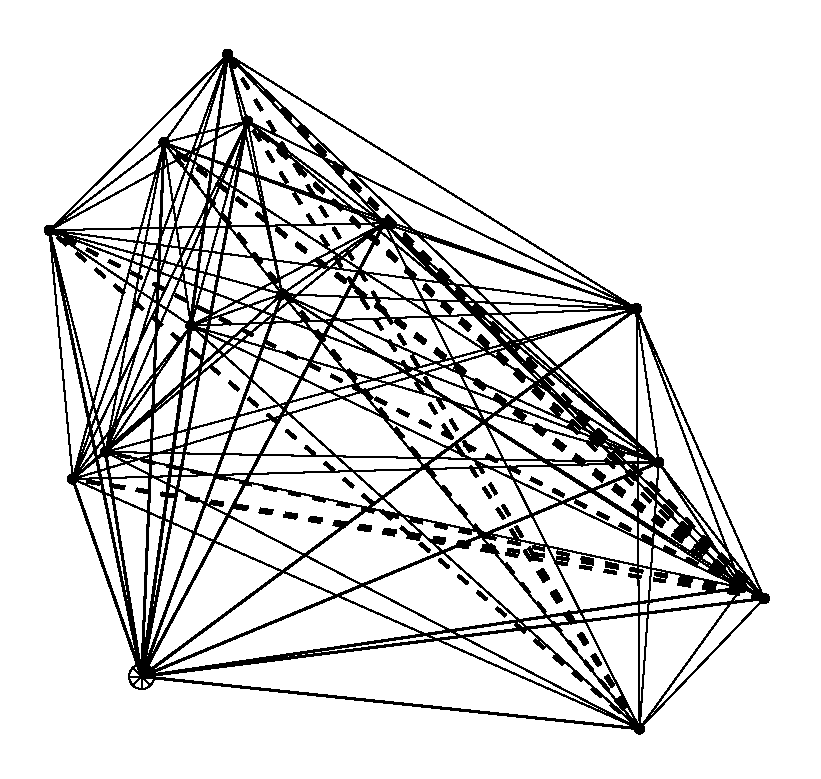
\includegraphics[width=0.4\textwidth]{DistEx.eps}\\
  \caption{GB-NLS 中的一步所涉及到的子图. 星型点: 未知点, 实心点:已知点.
  实线和粗实线: 已知的距离, 虚线: 计算的距离.}\label{fig:DistEx}
\end{figure}

在 GB-NLS 中, 首先是通过已知点的坐标计算
已知点之间未被测量的距离 (图 \ref{fig:DistEx} 中的虚线).
由此, 这 $l+1$ 个点所形成的子图, 其所有的两两距离都已知, 
从而可以利用 \ref{sec:MatDcomp} 中所介绍的矩阵分解算法来求解子问题.
求解之后需要通过旋转平移将这 $l+1$ 个点在子坐标系中的坐标变换到
原全局坐标系, 细节将在后文 (??) 给出.
这一步可以确定未知点 $j$, 与此同时对已经确定的 $l$ 个点进行微调. 
通常这个调节是细微的, 但是对整个算法却是非常重要的,
因为它提供了一个根据新利用到的距离改进原本不精确的定位的机会,
而不像在 GB-LLS 中, 一个点一旦被确定, 就永远地固定了.


\section{一些其他算法}
\label{sec:otheralg}






  %\include{chap/ouralg}
%  \include{chap/assess}
%  \include{chap/lfn}
%  \include{chap/sobolev}
%  \include{chap/subspace}
%  \include{chap/conclusion}

%  % 附录
%  \appendix

\chapter{引言}
\label{cha:introduction}
有许多种方式来描述距离几何问题, 我们采用图的语言. 

\begin{Prob}[等式约束的距离几何问题]
  对于图$G=(V,E)$, 其中$V$是顶点几何, $E$是边的集合, 给定每一条边 $(i,j)\in E$ 的长度为 $d_{ij}$, 求解$d$ 维欧式空间中的点的坐标 $\xn$,使得
\begin{equation}
  \|x_i-x_j\|=d_{ij}, \quad (i,j)\in E.
\end{equation}
\end{Prob}

在理想情况下, 给定的距离是没有误差(无噪音)的, 
此时问题叫做精确距离的距离几何问题, 否则称为不精确(带噪音)的距离几何问题.
一个更加实际的情形是, 给定的不是每一条边上的距离 $d_{ij}$, 
而是该距离的上界估计 $u_{ij}$ 和下界估计  $l_{ij}$.
此时问题变为求 $x_i\in \Real ^d$, 满足
\begin{equation}
  l_{ij}\leq \|x_i-x_j\| \leq u_{ij}, \quad (i,j)\in E.
\end{equation}
此时问题叫做给定上下界的距离几何问题.
在本文中, 我们会涉及到上下界的问题, 但重点研究带噪音的距离几何问题.


\section{距离几何问题的应用}
\label{sec:application}
距离几何问题在多个领域有着广泛的应用, 
本文仅列出其中最重要的几个例子, 实际应用包括但不限于这些.


\subsection{画图}
在画图 (Graph Drawing) 领域, 通常叫做图的实现(Graph Realization)问题~\cite{Gansner2005}.
在这个问题中, 我们的任务是画图使得点之间的距离满足事先给定的权重. 
这个问题跟我们后面提到的几个应用的区别是, 这些理论上的图
有时候会有多解的存在, 为了使画出来的图满足美观性的要求通常会引入其他约束条件.

\subsection{蛋白质折叠} 
这个术语翻译自 Protein Folding, 
在其他文献中也有被叫做蛋白质结构确定 (Protein Structure Determination)~\cite{Braun1987,Sit2011,Voller2013}, 
或是分子构象问题 (Molecular Conformation Problem)~\cite{Crippen1988,Biswas2008,Fang2013}, 
或是分子距离几何问题 (Molecular Distance Geometry Problem)~\cite{Dong2002,Dong2003,Carvalho2008}.

在这个问题中, 给定原子之间的部分距离, 我们需要给出蛋白质的三维结构.
在实际应用中, 这些距离通常是由实验测得的, 比如核磁共振(Nuclear Magnetic Resonace)
或X射线结晶技术(X-ray Crystallography), 或者通过一些生物学信息估算, 比如键长和键角.
在目前的应用中, 核磁共振是获得距离的主要技术.
由于蛋白质的很多重要性质都与三维结构紧密相关, 
所以这个问题非常具有实际意义.
    
\subsection{传感器网络定位} 
另一个非常重要的应用是传感器网络定位~\cite{Akyildiz2002,Chong2003,Mao2007,Yick2008}.
传感器非常便宜和方便, 它是用来环境监测, 动物管理等活动的一种有效的工具, 
甚至应用在军事行动中, 用于远程探测地面信息.
在这些应用中, 通常每一个个体都装备有传感器, 它可以用来
发射信号, 收集和简单地处理信息.
基于传感器的很多应用都是位置相关的, 它的第一步就是确定各个体的地理位置.
传感器能够在一定的射程内发射和接收信号, 这样附近的传感器就可以通过到达时间差
或信号的衰减来测量距离, 通常情况下后者更精确, 
对于前者来说时间同步是一大影响精度的因素.

这个应用更其他几个的一个重要差别是, 在此应用中, 小部分传感器结点的精确位置
是提前知道的, 这部分结点也被成为锚节点 (anchors).
在很多其他应用中, 结点的相对位置, 也就是整体结构,
但借助于这些锚节点, 传感器定位中可以得到个体的绝对位置.
 
\subsection{其他应用}
距离几何问题还有其他许多应用, 比如地下巷道定位.
在煤炭开采等地下巷道中, 由于卫星信号的缺失, GPS 这种常规定位手段就会失效.
如果让工人都携带传感器, 并在巷道中辅以锚节点, 
我们就能确定所有工人的位置, 这对日常管理和事故中的紧急救援都是非常有用的.

现今移动电子设备如手机等增长迅速, 我们可以大胆设想, 
在未来, 我们能够通过这些设备的近场通讯, 测量距离, 从而实现室内精确定位.
在一些大型商场中, 已经有些商家做到了这一点, 但主要是基于移动设备
跟锚节点的通讯来实现的. 未来如果移动设备也互相通信,
组成一个大的移动网络, 将有助于更快更精确地定位.

\subsection{一些注记}
在蛋白质折叠和传感器网络定位应用中, 由于核磁共振技术和无线信号强度
的限制, 我们能够测得的距离通常都是局部的.
这样, 从总体上来看, 我们已知的距离信息就是非常稀疏的,
这里稀疏的意义是, 已知的距离是所有的成对 (pairwise) 距离中的很小一部分.
这也是问题的一个难点所在, 关于这点我们会在后文的复杂性分析和数值实验中再深入讨论.

上面提到了不少应用, 这也是本文作者选择这个课题作为博士研究方向的出发点之一.
我们希望提出的算法不光要有理论上的意义, 也能真正用来解决实际问题.
尽管实际的应用问题要比理论研究复杂, 还需要考虑成本等实际因素,
但算法还是其中非常重要的一部分, 这正是我们努力的方向.

通过上面的讨论, 我们可以看到, 
尽管都叫做``距离几何问题'', 其具体形式可能在以下几个方面存在差异:
\begin{itemize}
  \item 是否存在锚节点~?
  \item 等式约束还是上下界约束~?
  \item 已知全部距离还是部分距离~?
\end{itemize}
问题形式的不同将导致截然不同的难度和求解算法.
另外强调一点, 我们假设需要求解的点所在空间的维数是确定的, 已知的.


 
\section{本文主要内容}

在本文中, 我们的目标是求解蛋白质折叠问题,
也就是, 不带锚节点, 等式约束, 
已知部分 (其实非常稀疏) 距离信息的三维空间的
距离几何问题.

%%%%%%%%%%%%%%%%%%%%%%%%%%%%%%%%%%%%%%%%%%%%%%%%%%%%%%%%%%%%%%%%%%%%%%%%%%%%%%%
%%%%%%%%%%%%%%%%%%%%%%%%%%%%%%%%%%%%%%%%%%%%%%%%%%%%%%%%%%%%%%%%%%%%%%%%%%%%%%%
\chapter{模型研究}
\label{cha:models}

\section{引言}
我们在第\ref{cha:introduction}章中介绍距离几何问题时, 
并不是将其描述为一个标准的优化问题, 而是一个非线性等式(不等式)问题.
但此问题一般是通过建模成一个优化问题来求解的, 这正是误差函数的角色.

我们观察到, 在已有的文献中, 不同的误差函数被提出和应用, 
大多基于作者自身的经验和偏好.
我们同时也发现, 不同的建模方式对算法有着或大或小的影响.
在我们自己研究中, 选择不同的误差函数也产生了截然不同的结果.
但这些在目前的文献中并没有得到系统的研究, 这正是本章的研究动机.
在本章中, 我们综述已有的误差函数, 分析其性质, 
并在此基础上提出了我们自己的误差函数.
新的误差函数有一些好的理论性质, 并在某些数值实验中得到了验证.

本章的结构如下. 
在 \ref{sec:oldfun} 中, 我们综述文献中存在的误差函数, 并分析其性质.
在 \ref{sec:newfun} 中, 我们提出几个新的误差函数.
\ref{sec:funnuc} 是一个简单的数值实验和对本章的总结.


\section{已有误差函数综述及分析}
\label{sec:oldfun}

\subsection{函数介绍}

我们首先考虑带等式约束的距离几何问题
\begin{equation*}
  \textrm{求~} \xn \in \Real^d, \textrm{~使得~} \|x_i-x_j\|=d_{ij}, \textrm{~对所有的~} (i,j)\in E.
  \leqno{(DGPe)}
\end{equation*}  
它可以按如下方式建模成一个无约束优化问题
\be \min_{\xn} f(\xn), \label{prob:error}\ee
其中, $x_i$ 是点的坐标, $f(\cdot)$ 是一个用来衡量计算距离和给定距离偏差的误差函数.
我们极小化误差函数, 使得求得的点之间的距离``尽可能''满足给定的距离.
这里``尽可能''是一个不精确的描述, 它的意义会在后文明确.

误差函数 $f$ 的选取, 在文献中有如下几种形式:
\begin{itemize}
  \item 应力函数 (Stress function)
  \be Stress(\xn) = \sum_{(i,j)\in E} \omega_{ij}(\|x_i-x_j\|-d_{ij})^{2}, \label{fun:stress}\ee
  \item 光滑应力函数 (Smoothed Stress function)
  \be SStress(\xn) = \sum_{(i,j)\in E} \omega_{ij}(\|x_i-x_j\|^2-d_{ij}^2)^{2},\label{fun:sstress}\ee
  \item 绝对误差函数 (Absolute Error function) 
  \be AbsErr(\xn) = \sum_{(i,j)\in E} \omega_{ij}\left|\|x_i-x_j\|^2-d_{ij}^2
   \right|, \label{fun:abserr}\ee
\end{itemize}
其中, $\omega_{ij}$ 是边 (i,j) 上的权重, 恰当地选取可以得到合适的模型.
例如, 我们可以选择所有的 $\omega_{ij}$ 为1, 平等对待所有距离数据, 
计算的是各项的绝对误差和;
我们如果有一些数据是否可信的先验信息, 就可以对值得信赖的距离项加大权重,
相反对不太确定的数据降低权重.
另一种特别的选择是在 (\ref{fun:stress}) 中选取  $\omega_{ij}=1/d_{ij}^2$ 
(相应的, 在 (\ref{fun:sstress}) 和 (\ref{fun:abserr}) 中分别为 $1/d_{ij}^4$ 及 $1/d_{ij}^2$), 
此时 (\ref{fun:stress}) 变为
\be Stress(\xn) = \sum_{(i,j)\in E} \left(\frac{\|x_i-x_j\|}{d_{ij}}-1\right)^{2}, \ee
误差函数衡量的就是相对误差. 

在实际应用中, 选择绝对误差还是相对误差函数, 要基于对数据误差来源的统计认识,
选择吻合的函数.
有些测量误差跟仪器有关, 跟距离的绝对大小没有关系, 这种情况下就选绝对误差函数;
反之, 若距离的误差跟其大小成正比, 则选择相对误差函数.

\subsection{性质分析}


\subsection{正则项}

\section{几个新的误差函数}
\label{sec:newfun}



\section{一个简单的数值实验}
\label{sec:funnuc}




关于距离几何问题的先驱性研究可以追溯到 Schoenberg 在 
1935年的研究~\cite{Schoenberg1935}, 
以及 Blumenthal ~\cite{Blumenthal1953} 和 Torgerson ~\cite{Torgerson1958} 的工作.
在那之后, 大量的算法被提出来了, 它们各有侧重, 各有优缺点. 
在这一章中, 我们首先综述一些误差函数, 


%%%%%%%%%%%%%%%%%%%%%%%%%%%%%%%%%%%%%%%%%%%%%%%%%%%%%%%%%%%%%%%%%%%%%%%%%%%%%%%
%%%%%%%%%%%%%%%%%%%%%%%%%%%%%%%%%%%%%%%%%%%%%%%%%%%%%%%%%%%%%%%%%%%%%%%%%%%%%%%
\chapter{已有算法综述}
\label{cha:algrev}

关于距离几何问题的先驱性研究可以追溯到 Schoenberg 在 
1935年的研究~\cite{Schoenberg1935}, 
以及 Blumenthal ~\cite{Blumenthal1953} 和 Torgerson ~\cite{Torgerson1958} 的工作.
关于已有工作的一个简单的总结, 请参考 \cite{Fang2013} 中的表13.1. 
在本章中, 我们综述一些我们关注的算法, 主要是跟我们的研究方向的, 
但不企图覆盖所有算法.

例如, \cite{Qi2012} 就是一篇我们略过的有趣的文章, 它基于关于距离矩阵的
一个著名的结果 \cite{Schoenberg1935}, 研究秩约束的既约(变形后的)的距离矩阵.
对于有更深入兴趣的读者, 我们推荐参考 Liberti, Lavor, Maculan 和 Mucherino 2014年
发表在 SIAM Review 上的综述性文章 \cite{Maculan2014}, 文章比较全面而详实,
几位作者都对距离几何问题有着多年的研究和关注.

本章的结构如下.
在 \ref{sec:MatDcomp} 中, 我们介绍一个老的很特殊的矩阵分解算法,
它只能用来求解已知所有距离的距离几何问题, 但是之后很多算法的基础.
在 \ref{sec:Continuation} 中, 我们介绍全局光滑算法, 它对原误差函数进行光滑化处理,
期望抹去不重要的局部极小值点, 保留真正的全局极小值点.
在 \ref{sec:SDPalg} 中, 我们介绍多个基于半定规划的算法. 
半定规划在近年来得到广泛而深入的研究, 距离几何问题是其一个典型的应用例子.
应用半定规划, 我们能够比较方便地处理带不等式约束的问题.
\ref{sec:GB} 是我们介绍的重点, 我们在下一章提出的新的算法就是基于这些已有的算法,
所以我们会多费笔墨介绍算法的细节.
最后, 在 \ref{sec:otheralg} 中, 我们简要地提到其他一些比较重要的算法.


\section{矩阵分解算法 (Matrix Decompostion Method)}
\label{sec:MatDcomp}

Blumenthal 在 \cite{Blumenthal1953} 中提出了矩阵分解算法来求解
全部距离已知的距离几何问题. 全部距离是指点与点之间的两两距离都已知.
据我们所知, 这是针对这一问题最老的成熟的算法.
尽管它只能用来求解这一特殊情形, 但由于它是后续多个算法的关键步骤,
它仍然是非常重要的, 故而我们在此给出这一算法的细节.

由于整个结构\footnote{Structure, 在本文中指由点和边组成的二维或三维图形, 强调相对位置.}
在刚性变换(包括平移,旋转,和反射)\footnote{在本文中, 均指代平移, 旋转和反射变换中的一个或多个的复合, 后文将不特别说明.} 下保持不变,
不失一般性, 我们设 $x_n$ 在原点, 也就是 $x_n = (0,0,0)^T$. 
我们有 $d_{in} = \|x_i-x_n\| = \|x_i\|$. 
更进一步, 我们对等式 $\|x_i-x_j\| = d_{ij}$ 的两边同时取平方, 得到
\be \|x_i\|^2 - 2x_i^Tx_j + \|x_j\|^2 = d_{ij}^2, \quad i,j = 1,2,\ldots,n-1.\ee
将式中的 $\|x_i\|$ 用 $d_{in}$ 替代, 
并且把所有已知项移到同一边, 我们有
\be\label{eqn:sqrdist} x_i^Tx_j = (d_{in}^2 - d_{ij}^2 + d_{jn}^2 )/2, \quad i,j = 1,2,\ldots,n-1.  \ee
令 $X=(x_1,x_2,\ldots,x_{n-1})^T$ 为坐标矩阵,
其中$X^T$ 的每一列是一个点的坐标.
令 $B = (b_{ij}) = ((d_{in}^2 + d_{jn}^2 - d_{ij}^2)/2)$ 为距离矩阵的一个变换.
通过这些记号, (\ref{eqn:sqrdist}) 中的所有等式可以写成一个更紧凑的形式
\be XX^T = B. \ee
上面这个矩阵方程可以按如下的方式通过奇异值分解
(Singular Value Decomposition, 简称 SVD) 来求解.

\begin{Thm}{(Eckart, Young \cite{Eckart1936})}
令 $B=U\Sigma\Tran U$ 为奇异值分解, 
其中 $\Sigma$ 是所有奇异值按降序排列形成的对角矩阵. 
令 $V=U(:,1:k)$ 以及 $\Lambda=\Sigma(1:k,1:k)$, 
我们有 
\be X = V\Lambda^{1/2} \label{SVDsolution} \ee 
是下面这个问题的解
\be \min_{rank(X)\leq k} \|X\Tran X-B\|_F. \ee
\end{Thm}

在我们的应用中, 如果所有的距离都是精确的, 
并且不是所有原子都在同一个平面上, 那么矩阵 $B$ 将是秩 3 的, 
(\ref{SVDsolution}) 给出的就是精确解.
如果某些距离带有误差, 那么 $B$ 的秩通常大于 3, 
(\ref{SVDsolution}) 得到的就是最佳秩 3 逼近.

对于已知全部距离的距离几何问题, 
Dong 和 Wu \cite{Dong2002} 第一次给出了一个线性时间的算法.
顺便一提的是, 这也是几何构建系列方法的第一篇文章,
尽管名字 ``Geometric Buildup'' 是在之后的文章 \cite{Dong2003} 正式提出的.
关于这个方法的详细情况将在 \ref{sec:GB} 中给出.


\section{全局光滑算法 (Global Continuation Algorithm)}
\label{sec:Continuation}
如前所述, 误差函数通常都有大量的局部极小值点,
所以要直接找到原函数的全局极小值点是非常困难的.
在 \cite{More1997,More1999} 中, Mor\'e 和 Wu 提出了
一个全局光滑算法 \emph{dgsol} 来客服这个困难,
它的主要思想如下所述.

首先, 对原函数应用一个全局光滑化步骤. 
具体来说, 我们计算原误差函数与高斯密度函数的卷积.
直观地看, 这个过程把原函数在某一点的值用它周围点的均值所替代,
取均值的权重由高斯密度函数所决定, 以该点为中心成正太分布.
经过这一过程, 很多局部极小值点都被抹去了, 而真正的全局极小值点则被保留下来,
所以要找到光滑化之后的函数的全局解就容易得多了.
函数光滑化的程度是由一个参数 $\lambda$ 所控制的,
当 $\lambda$ 趋近于 0 的时候, 光滑化的函数逼近原函数.

算法的第二个关键技术叫做延续 (continuation), 
即逐步减小参数 $\lambda$ 到 0, 将上一步得到的解作为下一步的初始值,
应用局部优化算法如梯度法回溯求解, 最终找到原问题的解.
这里的思想跟求解非线性系统中的``同伦算法''非常接近,
都是将原问题化成结构类似但简单得多的问题, 再逐步回溯, 最终求解到原问题.

在 \cite{More1999} 中, 作者们给出了算法在一些小的蛋白质片段 (fragment)
上的计算结果, 表明 \emph{dgsol} 比重启动 (multi-start) 算法要有效和可靠得多.
值得一提的是, 重启动算法依靠某种方式 (如随机) 选择不同的初值点,
最后找一个最好的点作为解输出, 是求解全局优化的常用算法. 

全局光滑算法在理论上非常有意思, 但想用该算法来求解大规模的实际问题,
还需要进一步的深入研究.


\section{基于半定规划的算法 (SDP based algorithms)}
\label{sec:SDPalg}
半定规划 (Semidefinite Programming, 简称 SDP) 是近些年优化领域的一个研究热点.
关于它的理论已经非常成熟, 并且有很多易用的开源软件被开发出来,
如 SeDuMi 和 SDPT3 等\footnote{关于 SDP 的文献, 软件, 通知等资料参考
\url{https://www-user.tu-chemnitz.de/~helmberg/semidef.html}}. 
据我们所知, 关于距离几何问题的半定松弛算法 (SDP relaxation) 
最早是由 So 和 Ye 在 \cite{So2006} 中提出的, 
在这之后被众多学者进一步研究 \cite{Biswas2006-1,Biswas2008,Shamsi2010,Fang2013}. 
我们在下文简单总结关于这个算法的关键技术.

这些算法用到的一个基本模型是 (\ref{fun:abserr}). 
将 $|x|$ 用两个变量替代为 $x_+-x_- ~(x_+\geq 0,~x_-\geq 0)$, 
从而消去了函数中的非光滑项.
令 $X\in \Real^{n\times d}$ 是前文提到的坐标矩阵,
则 (\ref{fun:abserr}) 中的 $\|x_i-x_j\|^2$ 项可以重写为 $e_{ij}^TXX^Te_{ij}$, 
其中 $e_{ij}=e_i-e_j$. 
令 $Y=XX^T$ ,并松弛成 $Y\succeq XX^T$ \cite{Boyd1994}, 
这个线性矩阵不等式等价于
\be Z=\left(\ba{cc} Y & X \\ X^T & I \ea \right) \succeq \textbf{0}, ~~Z \textrm{ 是对称矩阵}.\ee
这样, (\ref{fun:abserr}) 的半定松弛可以写成一个以 $Z$ 为变量的
标准的半定规划问题. 注意, 我们要求 $Z$ 矩阵右下角 $d \times d$ 的子矩阵为单位阵.

半定松弛算法一个主要的优点是, 将此算法从求解等式约束的问题
推广到处理不等式约束不存在本质的困难, 
而对于其他算法来说, 这种推广并不容易, 甚至是不可能的.

这个方法的一个主要困难在于, 由于目前求解器 (solver) 的限制,
求解大规模 (超过几千个变量) 的半定规划问题的计算开销非常大.
考虑到这一点, Biswas, Toh 和 Ye 在 \cite{Biswas2008} 中第一次提出了针对
距离几何问题的分布式 (distributed) SDP 算法.
他们利用距离信息是局部及稀疏的特点, 基于距离矩阵,
将原图分割成了若干个带有重叠 (overlap) 区域的子图.
从而将大规模问题化解为了一些可以较快求解的小规模问题,
再将各子块拼接起来, 得到原图的结构. 
这种分布式策略在 \cite{Fang2013} 中也被用到, 
文章中他们进一步结合了从化学知识推断出的其他距离信息, 
并且设计了启发式 (heuristic) 策略来检测子块是否被精确定位,
这在分布式算法中是很关键的一点.
除了分布式以外, 另一种克服此困难的方法是将半定松弛进一步松弛 \cite{Wang2008} 
成基于结点或基于边的子问题, 它们都是可以高效求解的小规模问题.



\section{几何构建算法 (Geometric Buildup Method)}
\label{sec:GB}

几何构建算法是 Dong 和 Wu 在 \cite{Dong2002} 中首次提出来的, 
针对的是已知全部距离的情形, 
随后被推广到处理稀疏数据 \cite{Wu2006}. 
该算法在 \cite{Wu2008,Sit2009} 中被进一步完善, 
线性和非线性最小二乘近似 (linear and nonlinear least square approximation)
被提出来防止误差的累积.

几何构建算法基于这样一个事实: 在 $d$ 维空间中,
一个点通常可以被 $d+1$ 个到该点的距离唯一确定.
例如, 在三维空间中, 两个到固定点的距离可以确定\footnote{意指未知点到固定点的距离要满足所给距离, 这样的点形成的集合.}
一个圆 (假设两圆相交但不相切); 
而三个距离一般可以确定两个点, 四个距离则可以唯一确定一个点.
当然, 我们要求原来的四个固定点不在同一个平面上.
一般地, 我们要求 $d+1$ 个固定点不在同一个超平面上.
基于这些观察, 我们很自然地就可以得到集合构建算法的核心思想:
先确定四个点, 在逐步一个一个地确定剩下的点.
为了文章的完整性, 以及为了便于讨论并在下一章给出我们的新算法,
我们在此给出该算法的详细步骤.

\subsection{确定最初的四个点}
我们暂时考虑已知的是精确距离的情形.
首先找到形成团 (clique) 的四个点, 团的意思是这些点所构成的子图是一个完全图,
也就是这些点之间的两两距离都已知.
注意到在平移, 旋转和反射变换下, 所有的距离都保持不变,
不失一般性, 我们把第一个点设为原点---$(0,0,0)^T$, 
第二个点位于 x 的正半轴\footnote{为了方便起见, 我们称三个坐标轴为 x, y z 轴.},
其坐标为 $(d_{12},0,0)^T$,
第三个点位于 xy 平面的第一象限,
再随意选定第四个点位于两种可能性中的一个. 
我们略过这些简单的几何计算细节, 它们也可以在 \cite{Dong2002} 中找到.

\subsection{构建 (Buildup) 步: 确定一个未知点}
如前所述已经确定的四个点叫做基准点, 
我们再依次确定剩下的点, 正如从几块基石上一砖一瓦地盖起高楼大厦.

我们在此给出一个构建步的细节. 
我们把坐标已经确定的点叫做已知点, 剩下的点叫做未知点.
前文已经提到, 我们需要至少四个到已知点的距离来确定一个未知点.
假定点 $j$ 是要被定位的点, 它到四个已知点 $x_i ~(i=1,2,3,4)$ 的距离已知, 
也就是说, 我们有
\be \|x_i-x_j\| = d_{ij}, \quad i = 1,2,3,4.\ee
对这些等式的两边取平方, 得到
\be \|x_i\|^2 - 2x_i^Tx_j + \|x_j\|^2 = d_{ij}^2, \quad i = 1,2,3,4. \ee
注意, 在这些方程中, $x_j$ 是变量, 而 $x_i$ 是已知的.
现在我们有四个方程, 我们依次用后一个方程减去前一个方程\footnote{这不是唯一的方式, \cite{Dong2003} 讨论了不同的减去方式, 
以及在实际计算中可能不同的数值稳定性. 
我们可以在这多种方式中选择最优的一种, 但计算量也会成培增加.},
得到
\be 2(x_{i+1}-x_i)^Tx_j =(\|x_{i+1}\|^2-\|x_i\|^2) - (d_{i+1,j}^2-d_{ij}^2),\quad i = 1,2,3. \label{eqn:Ab} \ee
令 $A$ 为一个矩阵, $b$ 为一个列向量, 其中
\be A = 2\left[\ba{c} (x_2-x_1)^T \\(x_3-x_2)^T\\(x_4-x_3)^T \ea \right],
~b=\left[\ba{c}(\|x_2\|^2-\|x_1\|^2)-(d_{2j}^2-d_{1j}^2)\\
(\|x_3\|^2-\|x_2\|^2)-(d_{3j}^2-d_{2j}^2)\\(\|x_4\|^2-\|x_3\|^2)-(d_{4j}^2-d_{3j}^2)\ea \right],\label{eqn:dataAb}\ee
则 (\ref{eqn:Ab}) 中的等式可以写成一种更紧凑的形式
\be Ax_j=b. \label{eqn:Axb} \ee
如果这些已知点不都在同一个平面上, 那么 $A$ 是非奇异的,
未知点可以被唯一确定, 其精确解为 $x_j=A^{-1}b$.

\subsection{线性最小二乘}\label{LLS}
如果给定的距离是带误差的, 那么仅仅利用四个距离, 
求解方程 $Ax_j=b$ 并不能给出一个精确的解.
事实上, 从错误的距离信息出发, 我们几乎永远不可能得到``正确的''解,
但我们还是希望得到一个尽可能准确的解.
一种自然的处理办法就是, 利用尽可能多的距离, 从而得到一个合理的解.

假设我们已知的是 $l ~(l\geq 4)$ 个距离, 
那么我们就可以不求解等式方程 (\ref{eqn:Axb}), 
而是求解一个线性最小二乘问题
\be \min_{x_j} \|Ax_j-b\|, \ee
其中, $A$ 和 $b$ 是按照 (\ref{eqn:dataAb}) 类似的方式构成的, 
但都有 $l-1$ 行. 
这就是 Wu, Wu 和 Yuan 在 \cite{Wu2008} 中提出的
带线性最小二乘的几何构建方法, 更具体的细节可以参看原文.
我们在本文中将此方法简记为 GB-LLS.

\subsection{非线性最小二乘}\label{NLS}
注意到, 在 GB-LLS 中, 只有未知点到已知点之间的距离
(图 \ref{fig:DistEx} 中的粗实线) 被用到,
但是我们通常还会知道一些已知点之间的距离 (图 \ref{fig:DistEx} 中的实线). 
为了用到这部分信息, 在 \cite{Wu2008} 中, 
作者们进一步提出了带非线性最小二乘\footnote{这里并不算严格意义的``最小二乘''问题, 此处是类比于前一个算法的叫法.}
的几何构建算法, 我们在本文中记为 GB-NLS.

\begin{figure}[htb!]
  \centering
  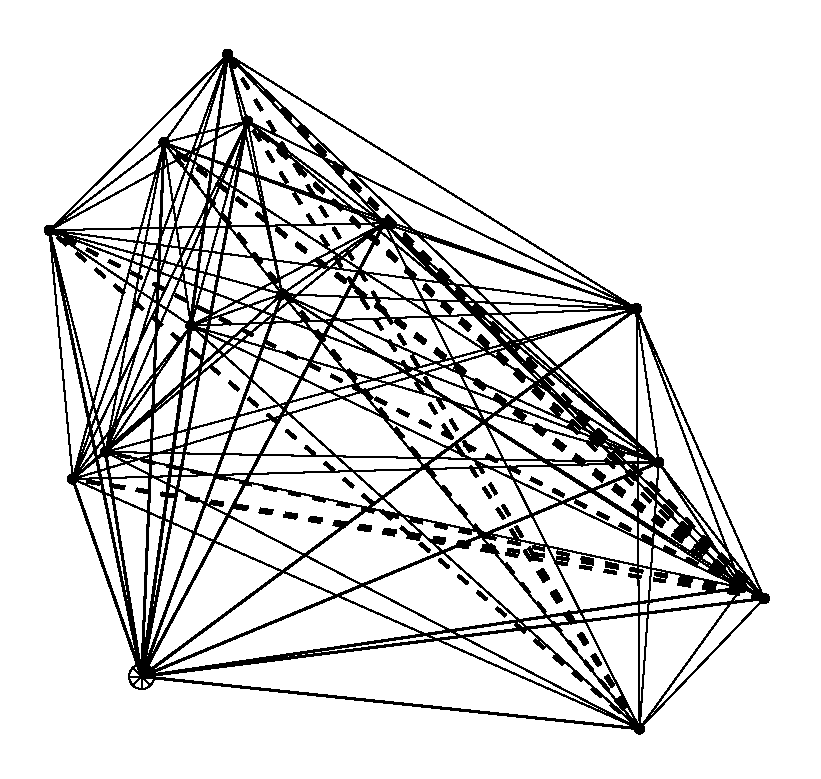
\includegraphics[width=0.4\textwidth]{DistEx.eps}\\
  \caption{GB-NLS 中的一步所涉及到的子图. 星型点: 未知点, 实心点:已知点.
  实线和粗实线: 已知的距离, 虚线: 计算的距离.}\label{fig:DistEx}
\end{figure}

在 GB-NLS 中, 首先是通过已知点的坐标计算
已知点之间未被测量的距离 (图 \ref{fig:DistEx} 中的虚线).
由此, 这 $l+1$ 个点所形成的子图, 其所有的两两距离都已知, 
从而可以利用 \ref{sec:MatDcomp} 中所介绍的矩阵分解算法来求解子问题.
求解之后需要通过旋转平移将这 $l+1$ 个点在子坐标系中的坐标变换到
原全局坐标系, 细节将在后文 (??) 给出.
这一步可以确定未知点 $j$, 与此同时对已经确定的 $l$ 个点进行微调. 
通常这个调节是细微的, 但是对整个算法却是非常重要的,
因为它提供了一个根据新利用到的距离改进原本不精确的定位的机会,
而不像在 GB-LLS 中, 一个点一旦被确定, 就永远地固定了.


\section{一些其他算法}
\label{sec:otheralg}



%%%%%%%%%%%%%%%%%%%%%%%%%%%%%%%%%%%%%%%%%%%%%%%%%%%%%%%%%%%%%%%%%%%%%%%%%%%%%%%
%%%%%%%%%%%%%%%%%%%%%%%%%%%%%%%%%%%%%%%%%%%%%%%%%%%%%%%%%%%%%%%%%%%%%%%%%%%%%%%
\chapter{新的基于几何构建的算法 (GBEM-LLS 和 GBEM-NLS) 及数值实验}
\label{cha:ouralg}

由于每一步涉及的都是小规模的易于求解的子问题, 相比于基于 SDP 松弛的算法, 
几何构建算法 (GB-LLS 和 GB-NLS) 非常快. 
然而, 已有的几何构建算法, 即便是最新的版本 \cite{Sit2009},
只能容忍数据中存在非常小的误差, 一般不超过 0.01\%, 
这使得该算法并不能很好地解决实际问题.
特别地, 即便是对于精确距离的情形, 当蛋白质中原子个数较多时 (多于几千),
舍入误差的累积 (error accumulation) 都会导致最终的结构完全偏离正确结果,
对于一般有误差的情形, 结果只会更糟.

这就是我们开始这项研究的最初的动机, 我们想要分析误差形成的原因,
并发展一些新的技术来客服误差累积的困难.
我们最终提出的算法可以看作是对已有几何构建算法的改进.
而另一个看待我们的算法的角度是, 
总的来看, 新的算法致力于求解一个误差函数极小问题, 我们的目标是求全局极小值点,
而问题却有特别多的局部极小值点, 所以我们要通过几何构建算法来去找一个好的初值点.
而从每一步来看, 我们解的是只跟很少项有关的子问题,
这也是借助了几何构建的思想.
总而言之, 为了使新算法快速而精确, 几何构建和优化过程同样地重要.

本章的结构如下. 
在 \ref{sec:ErrImportant} 中, 我们讨论为什么数值误差如此重要.
在 \ref{sec:ErrAnalysis} 中, 我们分析已有算法中, 误差的来源.
在 \ref{sec:CompOrder} 中, 我们给出一个有效的计算顺序策略.
在 \ref{sec:opt} 中, 我们讨论优化的子问题及其求解方法.
在 \ref{sec:framework} 中, 我们总结前述讨论, 给出算法的总体框架.
在 \ref{sec:NumResult} 中, 我们给出大量的数值实验结果, 并加以分析.
\ref{sec:summary} 是本章的总结.
最后, 在 \ref{sec:CodeWrite} 和 \ref{sec:ErrExample} 中, 
我们以附录的形式分别讨论算法的几个关键代码实现, 以及给出一个舍入误差累积的例子.

\section{为何数值误差很重要~?}
\label{sec:ErrImportant}

计算误差的累积是几何构建算法中的很严重的问题 \cite{Wu2006,Wu2008}, 
这在我们自己的数值实验中也得到了观察.
图 \ref{fig:OriginalOrder} 给出了一组典型的 RMSD\footnote{详细定义会在 \ref{sec:NumResult} 中给出, 在此可理解为所有点坐标的平均误差.} 结果,
这是将 GB-LLS 应用到计算蛋白质 1MQQ 得到的, 其中假设距离是精确的.
从理论上讲, 这个算法能够保证得到一个精确的蛋白质结构 \cite{Sit2009}. 
但是在实际计算中, 尽管 RMSD 在最开始的几百步非常好, 
可是它随着迭代的进行上升地非常快,
最后在差不多3500步的时候就完全错了.
这个例子表明, 算法 GB-LLS 在理论和数值表现上存在一个不可忽视的鸿沟,
这促使我们设计更加鲁棒 (robust) 的算法来解决这一问题.

\begin{figure}[htbp!]
  \centering
  \includegraphics[width=0.5\textwidth]{OriginalOrder.eps}\\
  \caption{将 GB-LLS 应用到计算蛋白质 1MQQ (5681个原子) 的 RMSD 结果 (距离是精确的, 距离阈值设为 6\AA). 结果经过了 $log10$ 函数换算, 表示的是 RMSD 的量级.}
  \label{fig:OriginalOrder}
\end{figure}


\section{已有几何构建算法的误差累积分析}
\label{sec:ErrAnalysis}
在这里我们考虑一种简单的情形, 也就是给定的距离都是精确的,
并且使用线性最小二乘来确定未知点. 
也就是说, 我们分析算法 GB-LLS 的一个迭代步.

假设点 $j$ 是要定位的未知点, 已知 $l$ 个到已知点 $1,2,\ldots,l$ 的距离. 
假设真实的坐标\footnote{我们可以固定最初确定的4个点为锚点, 剩下的点就可以用绝对坐标表示了.}
是 $\widehat{x}_i$, 而计算的坐标是 $x_i$, 
我们记该步之前点 $i$ 的定位误差为 $\delta x_i=x_i-\widehat{x}_i$,
并且进一步假设这些误差在同一个量级, 记为 $\delta x_i=O(\delta x)$.

我们需要求解最小二乘 $\min_{x_j} \|Ax_j-b\|$, 其中
\be A = 2[(x_{i+1}-x_i)^T], b=[(\|x_{i+1}\|^2-\|x_i\|^2)-(d_{i+1,j}^2-d_{ij}^2)],~i=1,2,\ldots,l-1.\ee
从而, 我们有
\begin{align}
  \|x_{i+1}\|^2-\|x_i\|^2 & = \|\widehat{x}_{i+1}+\delta x_{i+1}\|^2-\|\widehat{x}_i+\delta x_i\|^2    \\
  & = \|\widehat{x}_{i+1}\|^2-\|\widehat{x}_i\|^2 + 2\widehat{x}_{i+1}\delta x_{i+1} - 2\widehat{x}_i\delta x_i + \delta x_{i+1}^2-\delta x_i^2.
\end{align}
所以, $A=\widehat{A}+O(\delta x),~~b=\widehat{b}+O(\delta x)$, 进一步地, 
\begin{align}
  \|Ax_j-b\| & =\|(\widehat{A}+\delta A)(\widehat{x}_j+\delta x_j)-(\widehat{b} + \delta b)\| \\
  & =\|\widehat{A} \delta x_j + O(\delta x)\|.
\end{align}
从以上分析我们可以得出, 每一个构建步的误差主要来自三个方面:
\begin{enumerate}
  \item 从之前的计算中遗传下来的误差, 这些误差隐含在 $A$ 和 $b$ 中, 是构建步的主要误差来源.
  \item 由坏条件数 (ill-conditional) 的 $A$ 引起的计算误差, 这只会在很少的迭代步中占主导因素, 但有时会引起大的误差.
  \item 由有限精度计算带来的舍入误差.
\end{enumerate}

在计算中, 上述几种误差都是掺杂在一起的, 互相影响.
舍入误差我们无能为力, 所以我们的目标是设计算法避免坏条件数的 $A$,
并且尽量使之前的定位更加精确, 从而减小 $A$ 和 $b$ 中带来的误差.


\section{计算顺序: 选择新加入点的策略}
\label{sec:CompOrder}

\subsection{引言}
注意到几何构建算法是一个一个地确定所有点的坐标, 
并且依靠已知点的坐标和未知点到已知点的距离来决定未知点,
所以, 很显然, 先确定的点的精度将会对后续定位的点的精度产生重大影响.
这就是我们要考虑的计算顺序的问题.

在已有的几何构建算法中, 他们利用的是 PDB 文件\footnote{我们将在数值实验部分 \ref{sec:NumResult} 详细解释.}
中原子的默认顺序.
所以, 他们实际上隐式地利用了蛋白质的结构信息.
这种结构信息是有用的, 但在实际问题中是很难知道的, 
一般来说我们知道的只有距离信息 \cite{Dong2002}.
所以, 在本文中我们试图设计一种仅仅利用距离信息的规则,
这样会比较实际.

\subsection{新规则的定义和讨论}
基于以上分析和讨论, 我们提出利用以下两种信息来选择点 $j$ 作为未知点.
\begin{itemize}
  \item (结构信息)%: the largest number of known distances \\
  ~记 $\mathcal{Y}$ 是已知点的集合, $\mathcal{N} = \{1,2,\ldots,n\}\backslash \mathcal{Y}$ 是未被确定的点的结合, 我们定义
  \be p(i) = \sharp \{d_{ik}\neq 0: k\in \mathcal{Y}\}, ~~对所有的~i\in \mathcal{N}, \label{rule1} \ee
  并进一步定义
  \be \mathcal{I} = \{i: p(i) = \max_{k\in \mathcal{N}} ~p(k)\}, \label{rule2}\ee
  其中 $p(i)$ 是未知点 $i$ 到已经确定的点中已知距离的数目, $\mathcal{I}$ 是拥有最多的已知距离的未知点的集合.
  \item (距离信息)%: closest to the determined points \\
  ~我们选择点 $j$ 满足
  \be j = \arg\min_{i\in \mathcal{I}} \sum_{k\in \mathcal{Y}} d_{ik}, \label{rule3}\ee
  它是集合 $\mathcal{I}$ 中到已知点距离``最近''的点, 这里最近的意义是已知距离的和.
\end{itemize}

直观上看, 我们选择已知最多数目的距离, 并且离已知点最近的点.
在很多时候, 都会有多个点满足第一个规则, 所以我们需要第二个规则,
从而避免使算法不稳定或不可预测.

这个计算顺序的好处包括但不限于以下几个方面:
\begin{enumerate}
  \item 摇摆现象被消除了. 在已有的几何构建算法中, 我们经常观察到构建步会进行到离已知点整体比较远的地方, 再迭代回来. 在新的规则下, 这种来回摇摆的现象消失了.
  \item 作为前一点的结果是, 在往更远处迭代的时候, 通常已知点都是聚成团的, 其附近的点都已被确定, 这样在计算新的未知点的时候, 将会有更多的距离被用到. 更多的距离对提升算法的精准度和稳定性都是有帮助的.
  \item 整个算法更加稳定. 这里稳定的意义是, 这个规则下得到的系数矩阵 $A$ 的条件数通常都比较小, 求解线性最小二乘子问题的数值稳定性更好. 这一点在数值实验中得到了证实.
\end{enumerate}

\subsection{一个构造的简单例子}
在本节中, 我们构造了一个简单的二维例子, 如图 \ref{fig:CompOrder} 所示,
来说明计算顺序的重要性.
在这个例子中, 我们有6个点, 他们的序号和位置如图所示,
其中由点1和点2所决定的直线是水平的.
点之间已知的距离由实线表示.

\begin{figure}[htp]
  \centering
  \includegraphics[width=0.5\textwidth]{CompOrder.eps}\\
  \caption{一个简单的例子, 表明计算顺序的重要性}
  \label{fig:CompOrder}
\end{figure}

我们应用原始的 GB-LLS 来求解该问题. 
点 1,2,3 作为基准点首先被定位, 接着点 4,5,6 按次序一个一个被确定.
这个过程看起来非常完美, 但却暗含潜在的风险.
我们假设 $d_{34}$ 的测量不准确, 从而使得点4的定位在很小的扰动下到了水平线之下.
如果我们仅仅看前四个点, 结果还是可以接受的, 因为仅仅是第四个点有很小的误差. 
接着我们根据点1,2,4的位置定位点5,
它也将会定位在水平线之下, 从而产生非常大的误差.
最后, 点6也不能很好地被定位.
从代数上来看, 点4的小扰动使得点5的定位产生大的误差的原因是,
点 1,2,4 几乎在同一条直线上, 从而形成的系数矩阵 $A$ 是坏条件数的.

现在我们来看, 这种数值上的风险在我们的规则下是如何消失的.
最开始的两步跟原算法是一致的, 不同的是我们会先于点5确定点6,
因为他们都已知到确定点\pozhe 1,2,3,4 的三个距离, 但点6离它们(总距离)更近.
在点6被正确地定位后, 点5也就可以被很好地定位了,
因为此时我们可以利用四个距离, 而点1,2,4,6 可以形成一组稳定的基,
得到一个小条件数的 $A$.
这个人造的例子表明了我们的策略确实是有效的, 
在真实的蛋白质数据上的测试结果将在 \ref{sec:NumResult} 中给出.


\section{误差函数极小}
\label{sec:opt}
\subsection{子问题}
我们先介绍图论中诱导子图的概念. 
$G=(V,E)$ 是一个图, 其中 $V$ 是顶点集, $E$ 是边集.
$V'\subseteq V$ 是顶点集的一个子集, 
那么 $G(V')=(V',E')$ 就称为图 $G$ 的诱导子图, 
其中 $E'=\{(i,j)\in E: i\in V', j\in V'\}$.

在每一个构建步之后, 我们提出增加一个在子图 $G(j\cup N(j))$ 上的优化步, 
其中 $N(j)=\{k: d_{jk}\neq 0\}$ 是点 $j$ 的邻接点的集合. 
也就是说, 我们进一步求解以下子问题
\be \min  f(x_{j\cup N(j)}), \label{prob:sub}\ee
其中 $f(\cdot)$ 是定义在诱导子图 $G(j\cup N(j))$ 上的误差函数, 
未知距离\footnote{因为 $x_i$ 是要求解的坐标, 我们把 $\|x_i-x_j\|$ 称作未知距离.}到已知距离的偏差在边集 $E'$ 上被加和. 
%We choose $f(\cdot)$ as $Stress(\cdot)$ in (\ref{eqn:stress}) with $\omega_{ij}=1$ in this paper.

%\subsubsection{Comments and further discussion on error function}
注意到问题 (\ref{prob:sub}) 中的目标函数
与我们最终要求解的优化问题有着完全相同的形式,
但只包含集合 $j\cup N(j)$ 中点内部的距离.
由于实际问题中, 距离是稀疏而局部的 (sparse and local),
我们得到的是小规模的问题 (通常不多于几十个变量),
同时构建步可以提供一个高质量的初始点,
所以子问题 (\ref{prob:sub}) 通常可以在很少的迭代步之内被高精度地求解.
所以, 由增加的优化步所带来的计算量并不大.

从另一个角度来看, 考虑到距离信息的使用,
优化子问题可以看作线性最小二乘与非线性最小二乘的折衷.
就像我们之前提到的, GB-LLS 仅仅使用 $l$ 个距离\pozhe 太少,
GB-NLS 不但利用了已知的距离, 还利用了计算的距离\pozhe 太多, 
而我们在这两种极端方法中找了一个有效的折衷\pozhe 我们使用了
相关的全部距离, 但不使用计算出来的距离.
这样做的好处是多方面的.
我们既保留了 GB-NLS 的优点\pozhe 稳定性以及根据新加入的点和距离调整已知点的能力,
又克服了它的缺点, 避免了误差通过计算的距离而累积.
而且, GB-NLS 的关键步是使用矩阵分解算法,
是在变换后的距离矩阵上做运算,
而我们做的是误差函数极小化, 
更加符合原问题的本质\pozhe 距离尽可能地被满足.

\subsection{求解算法}
我们可以计算 $Stress$ 的导数如下所示,
\be \frac{\partial Stress}{\partial x_i}=2\sum_{j\in N(i)} \Big(1-\frac{d_{ij}}{\|x_i-x_j\|}\Big)(x_i-x_j), \label{gradient}\ee
其中 $N(i)$ 是 $i$ 的邻接点集合.

在本文中, 我们主要利用带 Barzilai-Borwein (BB) 步长 \cite{BB1988} 
的梯度法来求解 (\ref{prob:sub}). 
如果 BB 步连续 $M$ 次没有改进, 
我们也结合 Armijo 回溯线搜索 (backtracking line search) 来保证收敛性,
请参考 \cite{Armijo1966,Sun2006}.

\textbf{Armijo 回溯线搜索} ~令 $\alpha = \delta\beta^i$, 
其中 $\delta>0$ 是初始步长, 
$i$ 是满足下式的最小的非负整数
\be f(x)-f(x+\delta\beta^id)\geq -b\delta\beta^i d^T\nabla f(x), \ee
其中, $b\in (0,1)$ 是一个参数, $d$ 是搜索方向.

在迭代中, 
$\delta^k=\frac{\|s^{k-1}\|^2}{{s^{k-1}}^Ty^{k-1}}$ 是第$k$步的长 BB 步长, 
其中 $s^k=x^k-x^{k-1}$, $y^{k-1}=g^k-g^{k-1}$, 而 $x^k$ 是迭代点,
$g^k$ 是梯度. 
迭代格式如下
\be x^{k+1} = x^k + \alpha^kd^k.\ee

%We also apply the following nonmonotone line search technique to make our algorithm have to ability to escape from some not so good local minimizers.

\section{算法总框架}
\label{sec:framework}
在本节中, 我们对前几节的讨论作一个总结,
给出我们的算法 GBEM
的总体框架.
%
%\begin{algorithm}[H]
%\SetKwInOut{Input}{input}\SetKwInOut{Output}{output}
%\Input{A symmetric distance matrix $D$} %to specify part of the pairwise distances}
%\Output{index set of determined points and coordinate matrix $X$}
%%\vskip1mm
%Find a maximal clique that are not in the same plane\;
%Use Matrix Decomposition Method to determine these points\;
%%Repeat:
%
%\While{not all the points are determined}{
%Find point $j$ according to \reff{rule1}, \reff{rule2} and \reff{rule3}\;
%\eIf{$l=p(j)\geq 4 ~\&~ N(j) \textrm{ not in the same plane}$}
%{Determine $x_j$ by linear \reff{LLS} or nonlinear least square \reff{NLS}\;
%Adjust the locations of points $j\cup N(j)$ by solving \reff{prob:sub}.
%}
%{No more point can be uniquely determined\;
%Return the determined index set and coordinates, stop.}
%}
%\caption{Enhanced Geometric Buildup for sparse noisy anchor-free Distance Geometry Problem}
%\end{algorithm}

\begin{Alg} (GBEM \footnote{Geometric Buildup-based Error Minimization (简记为 GBEM), to solve sparse, noisy and anchor-free distance geometry problem.})
  \begin{adjustwidth}{1cm}{0cm}
    \begin{enumerate}[步1.]
      \item 找一个不是所有点都在同一个平面上的极大团, 利用矩阵分解算法 (\ref{sec:MatDcomp}) 确定这些点的坐标. 令 $\mathcal{T}=$ \{确定点的指标\}.
      \item 根据 (\ref{rule1}), (\ref{rule2}) 及 (\ref{rule3}) 找到指标 $j$. 如果 $l=p(j)\geq 4$, 且 $N(j)$ 中的点不都在同一个平面上, 转步3, 否则转步5.
      \item 用线性最小二乘 (\ref{LLS}) 或非线性最小二乘 (\ref{NLS}) 计算坐标 $x_j$, 并求解子问题 (\ref{prob:sub}), 调整 $x_{j\cup N(j)}$. 令 $\mathcal{T}=\mathcal{T}\cup \{j\}$.
      \item 如果所有点都已确定, 转步5, 否则转步2.
      \item 求解定义在 $\mathcal{T}$ 上的问题 (\ref{prob:error}), 停止.
    \end{enumerate}
  \end{adjustwidth}
%\caption{基于几何构建的误差极小算法 GBEM, 用来求解稀疏的带误差距离的, 无锚节点距离几何问题.}
  \label{alg:EGB}
\end{Alg}
根据步3中计算方法的不同, 我们把新提出的算法分别叫做
GBEM-LLS 和 GBEM-NLS.

%
%\subsection{Subspace point of view}
%Subspace is not a new concept but somehow a new aspect to view an algorithm \cite{Yuan2007}, and also useful philosophy to design algorithm to solve large-scale problems. We now focus the optimization problems solved in Algorithm \ref{alg:EGB} and explain this algorithm in subspace fashion.
%
%Our final task is to solve \reff{prob:error} (Step 5), which is an optimization problem with $n$ points thus totally $n\times  d$ variables. Instead of solving this difficult problem directly, we actually choose to iteratively minimize this function restricted at subspace $x_{j\cup N(j)}$ (Step 3), which is much easier to solve.
%
%\subsection{Convergence}
%The convergence of Algorithm \ref{alg:EGB} to a local minimizer is guaranteed by the standard theory of gradient method with Barzilai-Borwein step size \cite{BB1988,Sun2006}. However, as we have stated before, this local convergence is of little meaning in practice. On the other hand, the convergence to global solution is not easy to prove (actually, we believe there exist counterexamples, but this kind of example is meaningless for real applications, we do not waste our time to do that). Numerical results in next section will show that our algorithm can converge to global solution or very close to optimal solution in many instances.

\section{数值实验}
\label{sec:NumResult}
关于距离几何问题, 我们没有找到任何公开的测试数据集.
即使对于蛋白质折叠, 不同的文章使用的都是不同方式构造的模拟数据.
例如, 在 DAFGL \cite{Biswas2008} 中, 
作者使用了部分距离小于 6\AA ~(1\AA ~= $10^{-10}$m)~ 的上下界数据.
而在改进的 DISCO \cite{Fang2013} 中, 
20\% 的距离小于 6\AA 的带误差的数据被使用,
但作者结合了从化学知识推断出的其他距离信息.
所以, 想要把我们的算法跟已有的算法做一个直接的对比并不容易,
因为问题的设定并不完全相同, 而模拟数据的误差又是随机产生的.
在本文中, 我们将我们的算法跟已有的最新版本的几何构建算法 \cite{Sit2009} 作对比, 
尤其是展示新算法处理大误差数据的能力.

我们在 \ref{sec:ProbSet} 中介绍怎样构造测试数据集, 用来模拟真实的蛋白质数据.
在 \ref{sec:result} 中, 我们展示详细的数值结果, 
并且基于数值结果进行讨论分析, 给出一些结论.

\subsection{问题设定}
\label{sec:ProbSet}
我们先从蛋白质数据银行 (Protein Data Bank\footnote{\url{http://www.pdb.org}}, 
简称 PDB) \cite{Berman2000} 下载真实的蛋白质结构数据.
PDB 是一个由实验确定的三维蛋白质结构数据库, 
它包含蛋白质中的三维生物大分子结构数据.
根据 PDB 文件中原子的坐标, 我们使用圆盘图模型 (disk graph model) 来构造距离矩阵,
也就是说, 我们假设距离 $d_{ij}$ 是已知的, 
如果该距离小于或等于实现给定的距离阈值 
(cutoff, 通常为 5\AA ~或 6\AA, 其中 6\AA ~差不多是核磁共振技术
能够测量的两个原子之间的最大距离 \cite{Biswas2008}). 
通过这种方式, 我们模拟, 由于生物技术的限制,
只有小于一定阈值的距离才能够被测量这一真实情况.

在实际应用中, 测量到的数据通常都带有误差,
我们也在实验数据中通过添加正太分布或者均匀分布的乘性误差来模拟这一情况.
我们令测量到的距离 $d_{ij}$ 为
\be d_{ij} = \bar{d}_{ij}(1+\delta_{ij}*nl), \label{dij} \ee
其中, $\bar{d}_{ij}=\|\bar{x}_i-\bar{x}_j\|$ 是原子 $i$ 到原子 $j$ 之间的真实距离,
$\delta_{ij}$ 是一个遵从事先给定的分布的随机数.
例如, \cite{Biswas2008} 使用了标准正太分布 $\delta_{ij} \sim N(0,1)$,
而 \cite{Sit2009} 则使用了均匀分布 $\delta_{ij} \sim U[-1,1]$. 
我们在本文中汇报正态分布误差的结果, 
而略过在均匀分布上的结果, 对于我们的算法结果没有明显差别.
在 (\ref{dij}) 中,  $nl$ 是我们预先设定的误差水平,
在本文中等于 $1\%$, $5\%$, 或 $10\%$,
分别代表较小, 中等和较大的误差水平.

%\newcolumntype{R}{>{\flushright\arraybackslash}X}
%\renewcommand\arraystretch{0.85}
\setlength{\tabcolsep}{11.5pt}
\begin{table}[!htbp]
  \centering
  \footnotesize{
    \caption{测试问题信息汇总}
    \begin{tabular}{lrcccccccc}
      \toprule
      &  &  \multicolumn{4}{c}{cutoff = 5\AA} & \multicolumn{4}{c}{cutoff = 6\AA} \\
      \cmidrule(r){3-6}\cmidrule(r){7-10}
      \hd{ID}& \hd{Num} &  & \multicolumn{3}{c}{degree} &  & \multicolumn{3}{c}{degree}\\
      \cmidrule(r){4-6} \cmidrule(r){8-10}
      & & \hd{per} & max & min & avr &\hd{per} & max & min & avr \\
      \midrule
      1PTQ &  402 & 5.46 & 38 & 4 & 21.9 & 8.79 & 61 &  6& 35.3  \\
      1HOE &  558 & 4.05 & 38 & 6 & 22.6 & 6.55 & 65 & 11& 36.5  \\
      1LFB &  641 & 3.40 & 40 & 5 & 21.8 & 5.57 & 59 &  8& 35.7  \\
      1PHT &  811 & 3.35 & 48 & 5 & 27.1 & 5.37 & 75 &  7& 43.5  \\
      1POA &  914 & 2.51 & 39 & 4 & 22.9 & 4.07 & 67 &  8& 37.2  \\
      1AX8 & 1003 & 2.30 & 39 & 5 & 23.0 & 3.74 & 59 &  7& 37.5  \\
      4MBA & 1083 & 2.17 & 39 & 5 & 23.5 & 3.56 & 60 &  5& 38.5  \\
      1F39 & 1534 & 1.47 & 40 & 5 & 22.6 & 2.43 & 62 &  7& 37.2  \\
      1RGS & 2015 & 1.12 & 41 & 3 & 22.6 & 1.87 & 66 &  4& 37.7  \\
      1KDH & 2846 & 0.83 & 43 & 4 & 23.6 & 1.36 & 64 &  5& 38.8  \\
      1BPM & 3671 & 0.66 & 42 & 3 & 24.4 & 1.12 & 64 &  4& 40.9  \\
      1RHJ & 3740 & 0.65 & 40 & 4 & 24.4 & 1.10 & 61 &  5& 41.2  \\
      1HQQ & 3944 & 0.60 & 40 & 3 & 23.7 & 1.00 & 64 &  5& 39.5  \\
      1TOA & 4292 & 0.56 & 39 & 3 & 24.0 & 0.94 & 62 &  4& 40.1  \\
      1MQQ & 5681 & 0.44 & 44 & 5 & 25.2 & 0.75 & 66 &  7& 42.4  \\
      1HMV & 7398 & 0.32 & 42 & 3 & 23.3 & 0.52 & 67 &  4& 38.7  \\
      1I7W & 8629 & 0.29 & 48 & 3 & 24.7 & 0.47 & 73 &  5& 40.9  \\
      \toprule
    \end{tabular}\\[-3mm]
    \label{table:probinfo}
    \begin{flushleft}
      *ID---PDB 中蛋白质的ID, Num---蛋白质中原子的数目, per---已知的距离占所有的两两距离的百分比, degree---所有点的最大/最小/平均度
    \end{flushleft}
  }
\end{table}
我们用 GBEM-LLS 和 GBEM-NLS 计算文章 \cite{Biswas2008} 和 \cite{Sit2009}
用到的所有 17 个蛋白质, 其原子个数从 402 到 8629 不等. 
我们将测试问题的信息在表 \ref{table:probinfo} 汇总. 
表的第一列是 PDB ID, 它是蛋白质在 PDB 中独一无二的标识. 
第二列是每一个蛋白质中原子的个数, 也就是我们问题中点的个数. 
在第三列, 我们仿照 \cite{Biswas2008} 给出距离矩阵的稀疏度, 
它是已知的距离占所有的两两距离的百分比,
更稀疏的问题意味着我们知道``更少''的距离, 在一定程度上反映了问题的难度.
但是, 我们并不认为这是一个描述问题难度的很准确的标准.
比如, 假设我们将一个图复制 9 份, 并且增加少量必要的距离使得图形成一个刚性结构,
这样, 已知的距离差不多是 10 倍多 (呈线性增加), 
而总的两两距离的数目是平方量级的, 也就是说, 差不多 100 倍多, 
所以问题的稀疏度显著地增加了, 但问题的难度, 
除了存储和计算时间的考虑, 并没有显著地增加.
这个例子表明, 这个标准跟我们的直觉 \pozhe ``越稀疏的问题, 难度会显著增加''
并不是很吻合.
更准确地说, 当问题中点的数量差不多时, 稀疏度才是一个有意义的衡量问题难度的标准.
所以, 在本文中, 我们提出结合所有点的度 (degree) 的信息来说明问题的难度.
在 4--6 列中, 我们给出问题的最大, 最小和平均度.
我们将会看到, 度信息能更好地反映问题的难度, 尤其是对几何构建类的算法.
最后四列跟 3--6列是类似的, 不过把距离阈值从 5\AA ~增加到 6\AA,
也就是假设知道更多的距离信息.

我们的程序完全是用 Matlab 写的.
程序中最耗时的部分是循环计算梯度值, 
而这部分可以用 C 语言写, 并编译成 MEX 文件来加速,
但我们并没有这么做.
本节中所有的实验结果都是在 Dell 个人电脑上运行的,
其 CPU 为 2.83 GHz, RAM 为 4.00 GB, 
使用的程序版本为 Matlab R2013b, 8.2版.

\subsection{实验结果比较标准}
\label{sec:result}
我们将算法 GBEM-LLS 和 GBEM-NLS 应用到距离矩阵上.
注意, 我们的算法需要的唯一信息就是距离,
点的正确坐标仅仅是用来检验定位的精确度 (accuracy),
它是由如下定义的均方根偏差 (Rooted Mean Squared Deviation, 缩写为 RMSD\footnote{我们在后文还会见到其他相关的标准, 如函数值等, 但我们认为 RMSD 是衡量定位精度的最可信的标准. 在本文中, 我们所称的定位精度都是指 RMSD 值的大小.}) 来衡量的:
\be RMSD(X,Y) = \min_{Q,T}\{ \|Y-XQ-T\|_{F}/\sqrt{n}: \Tran{Q}Q=I\}, \ee
其中, $X\in \Real^{n\times 3}$ 和 $Y\in \Real^{n\times 3}$ 
分别是计算的和真实的坐标矩阵, 
$T$ 是平移向量, $Q$ 是正交矩阵.
粗略地讲, 我们通过刚性变换移动 $X$, 使其与 $Y$ 尽可能地吻合,
而 RMSD 衡量的就是移动后最小的偏差. 
需要特别注意的是, RMSD 仅能用来事后检验算法的表现,
并不能用来当作算法终止准则 (stopping criterion), 
因为它的计算要用到真实的坐标矩阵 $Y$,
而这是实际应用中是未知的.
事实上, 各种算法都是使用跟误差函数相关的量作为停机准则,
比如函数值, 或梯度模. 
其中文章 \cite{Biswas2008} 使用的一个终止准则定义如下:
\be LDME = \Big(\frac{1}{|E|} \sum_{(i,j)\in E}\big(\|x_i-x_j\|-d_{ij}\big)^2\Big)^{1/2}. \ee
但正如作者在文中指出的, 
LDME (Local Distance Matrix Error) 虽然在计算上更实际, 
但并不是一个很可靠的标准, 
更小的 LDME 值并不一定意味着更精确的定位 (尽管在很多例子中成立).
所以, 在前几个主要结果中, 我们没有列出函数值的相关结果, 
尽管我们使用误差函数值和梯度模作为优化步中的终止准则.

\subsection{计算顺序的影响}
\setlength{\tabcolsep}{5.5pt}
\begin{table}[!htbp]
  \centering
  \footnotesize{
    \caption{精确距离情形下的 RMSD (\AA) 结果}
    \begin{tabular}{lrcccccccc}
      \toprule
      &  & \multicolumn{4}{c}{cutoff = 5\AA}
      & \multicolumn{4}{c}{cutoff = 6\AA} \\
      \cmidrule(r){3-6} \cmidrule(r){7-10}
      \hd{ID} & \hd{Num} & \multicolumn{2}{c}{LLS} & \multicolumn{2}{c}{NLS} & \multicolumn{2}{c}{LLS} & \multicolumn{2}{c}{NLS} \\
      \cmidrule(r){3-4} \cmidrule(r){5-6} \cmidrule(r){7-8} \cmidrule(r){9-10}
      & & \hd{GB} & \hd{GBnew} & \hd{GB} & \hd{GBnew} & \hd{GB} & \hd{GBnew} & \hd{GB} & \hd{GBnew} \\
      \midrule
      1PTQ &  402 & 1.4e$+$00 & 6.5e$-$13 & 5.5e$-$14 & 5.1e$-$14 & 2.6e$-$09 & 2.8e$-$14 & 5.0e$-$14& 2.9e$-$14  \\
      1HOE &  558 & 5.8e$-$02 & 3.0e$-$13 & 1.6e$-$13 & 2.4e$-$14 & 3.1e$-$09 & 3.8e$-$14 & 2.7e$-$13& 2.0e$-$14  \\
      1LFB &  641 & 2.0e$-$02 & 9.3e$-$14 & 9.5e$-$14 & 3.1e$-$14 & 2.1e$-$10 & 4.6e$-$14 & 5.5e$-$14& 2.1e$-$14  \\
      1PHT &  811 & 1.2e$+$01 & 2.0e$-$12 & 1.1e$-$13 & 6.3e$-$14 & 8.2e$-$09 & 9.3e$-$14 & 1.8e$-$13& 5.7e$-$14  \\
      1POA &  914 & 6.6e$+$00 & 8.2e$-$13 & 3.2e$-$13 & 7.4e$-$14 & 1.9e$-$09 & 2.8e$-$13 & 1.5e$-$13& 4.7e$-$14  \\
      1AX8 & 1003 & 5.2e$+$00 & 1.1e$-$11 & 4.0e$-$13 & 3.3e$-$14 & 1.8e$-$05 & 5.4e$-$14 & 4.6e$-$12& 3.0e$-$14  \\
      4MBA & 1083 & 4.9e$+$00 & 3.6e$-$12 & 1.8e$-$13 & 8.2e$-$14 & 3.8e$-$06 & 1.2e$-$13 & 2.6e$-$13& 6.9e$-$14  \\
      1F39 & 1534 & 1.4e$+$00 & 6.7e$-$13 & 7.9e$-$13 & 5.2e$-$14 & 6.3e$-$08 & 2.1e$-$13 & 1.9e$-$13& 4.7e$-$14  \\
      1RGS & 2015 & 2.0e$+$01 & 2.5e$-$10 & 8.3e$-$12 & 2.2e$-$13 & 1.1e$-$01 & 2.1e$-$12 & 2.4e$-$12& 1.7e$-$13  \\
      1KDH & 2846 &     -     & 7.2e$-$11 &     -     & 1.9e$-$13 &     -     & 5.6e$-$13 &     -    & 1.5e$-$13  \\
      1BPM & 3671 & 6.4e$+$04 & 9.6e$-$10 & 8.1e$-$11 & 1.3e$-$13 & 3.6e$-$02 & 3.3e$-$13 & 1.0e$-$11& 1.0e$-$13  \\
      1RHJ & 3740 &     -     & 3.7e$-$09 &     -     & 6.4e$-$14 &     -     & 3.9e$-$13 &     -    & 8.2e$-$14  \\
      1HQQ & 3944 &     -     & 1.3e$-$09 &     -     & 5.3e$-$14 &     -     & 9.0e$-$13 &     -    & 6.8e$-$14  \\
      1TOA & 4292 &     -     & 3.4e$-$09 &     -     & 9.5e$-$14 &     -     & 4.9e$-$12 &     -    & 2.2e$-$13  \\
      1MQQ & 5681 &     -     & 6.8e$-$11 &     -     & 1.6e$-$13 &     -     & 6.1e$-$13 &     -    & 6.8e$-$14  \\
      1HMV & 7398 & 1.2e$+$03 & 6.1e$-$07 & 1.1e$-$08 & 3.8e$-$13 & 3.5e$+$01 & 5.6e$-$11 & 5.5e$-$07& 6.0e$-$13  \\
      1I7W & 8629 &     -     & 2.0e$-$06 &     -     & 3.8e$-$13 &     -     & 6.4e$-$12 &     -    & 2.7e$-$13  \\ \toprule
    \end{tabular}\\[-4mm]
    \label{table:exact}
    \bl *ID---PDB 中蛋白质的ID, Num---蛋白质中原子的个数, LLS---线性最小二乘, NLS---非线性最小二乘, GB---原始的几何构建算法, GBnew---加入了新的计算顺序规则的几何构建算法(但未加入优化步), '-'表示该例子在 \cite{Sit2009} 中未被测试 \el
  }
\end{table}

我们首先测试新定义的计算顺序规则的效果.
我们将已有的几何构建算法记为 GB, 
而把加入了新定义的计算顺序规则的算法记为 GBnew.
注意在 GBnew 中, 我们没有考虑优化步,
它与 GB 的唯一不同就是选择新加入点的规则不同, 
我们以这种方式来考察新规则的效果.

数值实验的 RMSD 结果如表 \ref{table:exact} 所示, 
其中关于 GB 的结果来源于 \cite{Sit2009} 的表 2 和表 3, 
而~'-' 表示相关蛋白质未被测试. 
从表格中, 我们可以看出 GBnew 总是能比原算法得到更好的结果.
特别是在数据比较稀疏的情况下 (cutoff=5\AA), 
对于不少蛋白质原算法都不能得到一个很好的结果,
但我们的算法可以.
我们也像 \cite{Sit2009} 测试了阈值为 7\AA ~和 8\AA~的情况, 
所有的测试例子都可以被精确定位, 即使是那些原算法不能确定的.
但这种阈值设定并不是很切合实际, 而结果也类似, 所以在此不给出详细结果.
另外, 由新规则带来的计算时间的增加相对于原算法几乎是可以忽略的.
比如, 一个有 8629 个原子的蛋白质---1I7W, 当阈值设为 6\AA ~时,
可以被 GBnew-LLS 在 19.0 秒内确定结构.

在给出更多的数值结果之前, 我们必须指出,
数值结果是跟程序设定的参数相关的.
一般来说, 最大迭代步和梯度模终止准则精度的不同 (例如, $10^{-2}$ 还是 $10^{-3}$) 
都会得到不同的 RMSD 和 CPU 时间结果. 
在绝大多数情况下, 更高的精度和更大的最大迭代步会得到更精确的 (也就是更小的 RMSD)
结果, 当然花费的时间更长.
但这并不绝对, 我们观察到的一个反例是,
对于 1MQQ (阈值为 5\AA, 误差水平为 5\%), 
我们将终止准则从 $10^{-2}$ 提高到 $10^{-3}$, 
我们得到了更小的误差函数值, 但 RMSD 却更大, 当然花费更多的时间.
这个例子也再次反映了函数值跟 RMSD 之间并不完全一致的关系,
所以我们需要在实践中总结经验, 选择一个合适的终止准则精度, 
一味地追求更小的目标函数值并不总是值得.
关于参数设定还有一点值得说明.
一般来说, 对于某个特定的蛋白质数据, 我们总可以调整参数得到更好的结果,
但我们并没有那么做, 因为在实际应用中, 
我们总是需要先对算法设定参数, 再去计算, 而不是反过来.
在本文中, 所有的数值结果都是用同样的参数得到的.

\setlength{\tabcolsep}{6pt}
\begin{table}[!htbp]
  \centering
  \footnotesize{
    \caption{阈值为 5\AA 时的 RMSD (\AA) 和 CPU 时间 (秒), 误差水平为 1\% 和 5\%}
    \begin{tabular}{lrrrrrrrrrr}
      \toprule
      & & & \multicolumn{4}{c}{noise level = 1\%}
      & \multicolumn{4}{c}{noise level = 5\%} \\
      \cmidrule(r){4-7} \cmidrule(r){8-11}
      \hd{ID} & \hd{Num} & \hd{nDet}& \multicolumn{2}{c}{LLS} & \multicolumn{2}{c}{NLS} & \multicolumn{2}{c}{LLS} & \multicolumn{2}{c}{NLS} \\
      \cmidrule(r){4-5} \cmidrule(r){6-7} \cmidrule(r){8-9} \cmidrule(r){10-11}
      & & & \hd{RMSD} & \hd{CPU} & \hd{RMSD}  & \hd{CPU} & \hd{RMSD}  & \hd{CPU} & \hd{RMSD}  & \hd{CPU} \\
      \midrule
      1PTQ &  402 &  402 & 1.1e$-$01 &  1.0 & 6.0e$-$02 &  1.1 & 2.0e$-$01 &   2.1 & 2.1e$-$01&   2.2  \\
      1HOE &  558 &  558 & 1.6e$-$01 &  1.7 & 3.7e$-$02 &  1.6 & 1.9e$-$01 &   3.6 & 2.6e$+$00&   4.1  \\
      1LFB &  641 &  641 & 1.6e$-$01 &  1.9 & 9.6e$-$02 &  1.9 & 5.9e$-$01 &   3.1 & 3.6e$+$00&   4.7  \\
      1PHT &  811 &  806 & 2.2e$-$01 &  2.6 & 6.1e$-$02 &  3.0 & 3.2e$-$01 &   6.0 & 1.9e$-$01&   5.8  \\
      1POA &  914 &  914 & 2.0e$-$01 &  2.9 & 8.8e$-$02 &  2.7 & 2.5e$-$01 &   6.4 & 4.1e$-$01&   5.9  \\
      1AX8 & 1003 & 1003 & 2.3e$-$01 &  3.8 & 7.9e$-$02 &  3.3 & 4.3e$-$01 &   8.8 & 8.0e$+$00&  10.8  \\
      4MBA & 1083 & 1080 & 2.1e$-$01 &  3.6 & 1.5e$-$01 &  4.3 & 2.6e$-$01 &   9.2 & 2.4e$+$00&  10.7  \\
      1F39 & 1534 & 1534 & 3.4e$-$01 &  5.2 & 1.3e$-$01 &  5.0 & 6.3e$-$01 &  12.7 & 5.1e$-$01&   9.5  \\
      1RGS & 2015 & 2010 & 9.5e$-$01 & 10.2 & 1.8e$-$01 &  7.2 & 2.9e$+$00 &  17.7 & 7.9e$+$00&  20.9  \\
      1KDH & 2846 & 2846 & 3.4e$-$01 & 17.7 & 2.3e$-$01 & 17.0 & 2.6e$+$00 &  28.5 & 1.4e$+$01&  34.6  \\
      1BPM & 3671 & 3668 & 4.5e$-$01 & 23.3 & 9.5e$-$02 & 16.4 & 7.4e$-$01 &  35.4 & 2.6e$-$01&  32.7  \\
      1RHJ & 3740 & 3740 & 1.3e$-$01 & 18.2 & 9.4e$-$02 & 18.5 & 4.4e$-$01 &  36.8 & 1.4e$+$01&  50.5  \\
      1HQQ & 3944 & 3938 & 1.7e$-$01 & 19.0 & 1.0e$-$01 & 17.5 & 4.3e$-$01 &  37.2 & 4.5e$-$01&  34.6  \\
      1TOA & 4292 & 4280 & 4.0e$-$01 & 29.4 & 1.2e$-$01 & 22.4 & 1.0e$+$00 &  43.6 & 5.1e$-$01&  34.4  \\
      1MQQ & 5681 & 5681 & 3.3e$-$01 & 47.8 & 1.0e$-$01 & 35.0 & 5.1e$+$00 &  70.2 & 3.6e$+$00&  73.0  \\
      1HMV & 7398 & 7389 & 2.6e$+$00 & 70.7 & 3.8e$-$01 & 54.3 & 3.7e$+$00 &  83.0 & 9.7e$+$00& 100.3  \\
      1I7W & 8629 & 8624 & 1.9e$+$00 & 79.0 & 1.0e$+$00 & 69.8 & 2.3e$+$01 & 109.4 & 6.2e$+$00& 121.1  \\ \toprule
    \end{tabular}\\[-4mm]
    \label{table:cut5}
    \bl *ID---PDB中蛋白质的ID, Num---蛋白质中原子的个数, nDet---被我们的算法确定坐标的原子个数, LLS---GBEM-LLS, NLS---GBEM-NLS, RMSD---计算的结构跟正确结构相比的RMSD值, CPU---算法定位过程花费的 CPU 时间 \el
  }
\end{table}

\subsection{主要数值结果}
我们在表 \ref{table:cut5} 中报告第一组针对大误差距离的实验结果,
其中距离阈值 5\AA, 误差水平设为 1\% 和 5\% 
(后者已有个别结果不太准确, 所以我们没有测试更大的误差水平). 
注意到有些蛋白质中,  nDet 列 (最终被定位的原子的个数) 的值 
要比蛋白质中原子的数目--- Num 略小,
也就是说对这些蛋白质而言, 我们的算法会有极少量的原子无法定位,
这是因为其距离矩阵过于稀疏, 使得有少量原子至多存在3个到已定位原子的距离,
所以存在至少两种可能的位置, 故不能唯一地被定位 
(当然我们也可以任意输出这些可能位置中的一个, 但目前我们只给出能唯一确定的原子的位置). 这是由问题本身的难度造成的, 并不是我们算法的缺陷.
表中报告的 RMSD 和 CPU 时间的结果都是针对确定点而言的.

当阈值设为 5\AA 的时候, 如果 RMSD 的值在 $10^{-1}$ 或者更小,
说明定位是非常精确的.
但如果超过 2\AA, 甚至更大的时候, 就可以算作不精确甚至是错误的了.
从表 \ref{table:cut5} 中也可以看出, 当误差比较小--- 1\%的时候,
GBEM-NLS 能够产生比 GBEM-LLS 更精确的结果, 
当误差增至 5\% 的时候, 结果是相反的.
类似的现象也在 \cite{Sit2009} 中被观察到.
这是因为, 当距离矩阵非常稀疏的时候, 
NLS 计算了很多已知点中未被测量的距离, 从之前的迭代步中继承了太多的误差,
最后导致结果不够准确.
总而言之, 在表中的两种情况下, 我们的算法能够确定大部分的蛋白质结构,
但也存在个别结构特别的蛋白质, 当误差过大的时候,
也会产生不精确甚至错误的输出.

至于 CPU 时间, 两个算法都能在几十秒的时间内确定几千个点的坐标.
甚至是对于最大的有 7398 和 8629 个原子的蛋白质,
只需要 100 秒左右的时间来定位, 这比一般的 SDP 类的算法要快得多\footnote{不是在同一个电脑上计算, 不算严格的比较, 但考虑到数量级的差别, 我们认为可以这一下断语.} \cite{Biswas2008}. 
另一个现象是, 如果两个算法都可以精确地定位,
一般来说 GBEM-NLS 的计算时间要比 GBEM-LLS 略少.
这是因为, NLS 产生了更精确的输出, 从而为优化步节省了时间.


\setlength{\tabcolsep}{3.5pt}
\begin{table}[!htbp]
  \centering
  \scriptsize{
    \caption{阈值为 6\AA~时的 RMSD (\AA) 和 CPU 时间 (秒), 误差水平为 1\%, 5\% 和 10\%}
    \begin{tabular}{lrrrrrrrrrrrrr}
      \toprule
      & & \multicolumn{4}{c}{noise level = 1\%}
      & \multicolumn{4}{c}{noise level = 5\%} & \multicolumn{4}{c}{noise level = 10\%} \\
      \cmidrule(r){3-6} \cmidrule(r){7-10} \cmidrule(r){11-14}
      \hd{ID} & \hd{Num} & \multicolumn{2}{c}{LLS} & \multicolumn{2}{c}{NLS} &
      \multicolumn{2}{c}{LLS} & \multicolumn{2}{c}{NLS}  & \multicolumn{2}{c}{LLS} & \multicolumn{2}{c}{NLS} \\
      \cmidrule(r){3-4} \cmidrule(r){5-6} \cmidrule(r){7-8} \cmidrule(r){9-10}
      \cmidrule(r){11-12} \cmidrule(r){13-14}
      & & \hd{RMSD} & \hd{CPU} & \hd{RMSD}  & \hd{CPU} & \hd{RMSD}  & \hd{CPU}
      & \hd{RMSD}  & \hd{CPU} & \hd{RMSD}  & \hd{CPU} & \hd{RMSD}  & \hd{CPU}\\
      \midrule
      1PTQ &  402 & 4.1e$-$02 &  1.3 & 3.4e$-$02 &   2.2 & 1.6e$-$01 &   2.8 & 1.9e$-$01&   4.3 & 3.1e$-$01 &   4.2 & 3.2e$-$01&   5.8  \\
      1HOE &  558 & 2.8e$-$02 &  1.9 & 2.3e$-$02 &   3.1 & 1.1e$-$01 &   4.2 & 1.0e$-$01&   6.3 & 2.1e$-$01 &   5.9 & 2.0e$-$01&   9.1  \\
      1LFB &  641 & 4.2e$-$02 &  2.2 & 3.8e$-$02 &   3.5 & 1.6e$-$01 &   4.8 & 1.7e$-$01&   8.6 & 3.3e$-$01 &   7.3 & 3.6e$-$01&   8.7  \\
      1PHT &  811 & 1.3e$-$01 &  3.4 & 4.8e$-$02 &   6.7 & 2.2e$-$01 &   7.3 & 1.6e$-$01&  14.7 & 4.8e$-$01 &  10.4 & 4.7e$-$01&  14.4  \\
      1POA &  914 & 4.2e$-$02 &  3.3 & 3.7e$-$02 &   5.8 & 1.7e$-$01 &   7.4 & 4.6e$-$01&  14.1 & 5.0e$-$01 &  10.0 & 5.3e$-$01&  13.9  \\
      1AX8 & 1003 & 5.8e$-$02 &  4.0 & 3.7e$-$02 &   6.2 & 1.3e$-$01 &   8.4 & 1.2e$-$01&  11.9 & 2.3e$-$01 &  11.9 & 2.9e$-$01&  16.2  \\
      4MBA & 1083 & 6.4e$-$02 &  4.8 & 2.9e$-$02 &   7.0 & 1.7e$-$01 &   9.2 & 1.2e$-$01&  13.0 & 2.6e$-$01 &  13.4 & 2.4e$-$01&  19.1  \\
      1F39 & 1534 & 4.6e$-$02 &  6.2 & 3.9e$-$02 &   9.7 & 2.5e$-$01 &  14.0 & 1.8e$-$01&  19.3 & 6.1e$-$01 &  18.1 & 3.5e$-$01&  24.0  \\
      1RGS & 2015 & 1.2e$-$01 &  8.6 & 5.1e$-$02 &  13.6 & 2.9e$-$01 &  18.4 & 2.8e$-$01&  27.2 & 6.0e$-$01 &  29.1 & 4.5e$-$01&  37.3  \\
      1KDH & 2846 & 1.0e$-$01 & 15.2 & 5.3e$-$02 &  22.7 & 1.6e$-$01 &  29.0 & 1.9e$-$01&  40.9 & 3.9e$-$01 &  43.0 & 1.2e$+$00&  51.2  \\
      1BPM & 3671 & 9.4e$-$02 & 20.5 & 3.7e$-$02 &  34.0 & 1.5e$-$01 &  41.4 & 1.4e$-$01&  67.8 & 2.4e$-$01 &  56.0 & 2.8e$-$01&  73.0  \\
      1RHJ & 3740 & 8.1e$-$02 & 22.0 & 2.8e$-$02 &  35.0 & 1.3e$-$01 &  39.9 & 1.2e$-$01&  59.0 & 2.5e$-$01 &  58.3 & 2.8e$-$01&  72.2  \\
      1HQQ & 3944 & 5.8e$-$02 & 20.5 & 3.7e$-$02 &  36.2 & 1.8e$-$01 &  43.0 & 1.9e$-$01&  63.4 & 3.4e$-$01 &  60.3 & 3.6e$-$01&  82.7  \\
      1TOA & 4292 & 8.4e$-$02 & 24.6 & 4.6e$-$02 &  45.3 & 1.8e$-$01 &  48.2 & 1.5e$-$01&  72.3 & 5.6e$-$01 &  72.8 & 4.2e$-$01&  89.2  \\
      1MQQ & 5681 & 4.0e$-$02 & 35.5 & 3.2e$-$02 &  64.8 & 1.1e$-$01 &  67.7 & 1.2e$-$01& 109.1 & 2.3e$-$01 &  94.4 & 2.7e$-$01& 129.0  \\
      1HMV & 7398 & 1.4e$-$01 & 57.7 & 1.0e$-$01 &  91.6 & 3.0e$-$01 & 105.9 & 4.0e$-$01& 146.0 & 1.2e$+$00 & 132.5 & 5.8e$-$01& 189.5  \\
      1I7W & 8629 & 2.9e$-$01 & 64.5 & 9.3e$-$02 & 111.7 & 7.9e$-$01 & 120.4 & 3.7e$-$01& 175.6 & 3.8e$+$00 & 165.7 & 6.7e$-$01& 225.1  \\
      \toprule
    \end{tabular}\\[-4mm]
    \label{table:cut6}                                                                  \bl *表中所有记号与表 \ref{table:cut5} 相同. \\
    *所有点都被唯一确定了, 所有没有 nDet 一栏.
    \el
  }
\end{table}

阈值为 6\AA~时的数值结果如表 \ref{table:cut6} 所示, 
我们考虑了不同的误差水平, 其中 10\% 可以算作非常大的误差了.
实验中所有的原子都能够被唯一定位, 因为最小度大于或等于4.
从表中我们可以看出, 两个算法都几乎可以非常精确地重构所有的蛋白质,
即使是误差水平大到 10\% 的时候, 除了三个 RMSD 略大的例子 
(其中两个1.2 的也还可以接受).
尤其值得注意的是, GBEM-NLS 能够非常精确地定位最大的几个测试例子.

基于表 \ref{table:cut5} 和表 \ref{table:cut6}, 
我们作出以下几个结论. 
\begin{enumerate}
  \item 对于蛋白质折叠问题, 我们的算法对大部分实例而言都是快速而精确的.
  \item 算法对误差有很好的鲁棒性, 尤其是距离信息稍多 --- 阈值为6\AA 的时候
  (从整体上看还是非常稀疏的).
  \item 距离相对较多 (这里的多寡是相对的, 跟具体的问题有关. 对于蛋白质折叠问题, 可以参看文章的实验结果, 阈值为6\AA ~可以认为是多, 阈值为5\AA ~可以算作少) 的时候, 推荐使用 GBEM-NLS 来实现高精度定位, 否则推荐 GBEM-LLS.
\end{enumerate}

在本小节的最后部分, 我们在表 \ref{table:fval} 中给出两组目标函数值,
从而对算法的效率有更深的认识.
其中一组记为 \emph{Fcomp}, 是 GBEM-NLS 算法停止时的目标函数值;
另一组记为 \emph{Ftrue}, 是将真实坐标带入目标函数得到的值.
注意到, 这时候目标函数中使用的是有误差的距离数据,
故 \emph{Fture} 的值不为 0.
令我们也略感惊讶的是, 除了 1KDH 这个没有被精确定位的个例, 
\emph{Fcomp} 甚至比 \emph{Ftrue} 要小.
.
这组结果表明, 我们的算法得到的结果几乎是最优了,
因为计算值甚至比``真实值''更小.
这组结果同时表明, 如果仅仅考虑距离信息, 在当前的模型下,
这差不多是我们能都得到的最好的结果了.
当然, 我们相信在模型上还有改进的空间, 这也是未来的一个有趣的研究方向.

\setlength{\tabcolsep}{5.5pt}
\begin{table}[!htbp]
  \centering
  \footnotesize{
    \caption{计算的目标函数值与``真实值''的比较 (阈值为 6\AA, 误差水平为 10\%)}
    \begin{tabular}{lrrrrrrrrr}
      \toprule
      ID    & 1PTQ & 1HOE & 1LFB & 1PHT & 1POA & 1AX8 & 4MBA & 1F39 & 1RGS \\
      \midrule
      Fcomp & 308.44 & 430.74 & 498.13 & 786.12 & 746.17 & 804.56 &  900.50	& 1256.29 & 1673.50 \\	
      Ftrue & 369.81 & 515.73 & 593.65 & 906.38	& 878.44 & 958.83 & 1069.63	& 1497.36 & 1984.83	\\
      \midrule
      \midrule
      ID & 1KDH & 1BPM & 1RHJ & 1HQQ & 1TOA & 1MQQ & 1HMV & 1I7W & \\
      \midrule
      Fcomp & 2844.25 &3437.47&	3540.00&	3528.73 & 3906.33 & 5503.48	& 6564.94 & 7934.25 & \\
      Ftrue & 2839.00 &4019.67&	4120.30&	4147.49 & 4560.61 &	6384.25 & 7524.43 &	9262.98 & \\
      \toprule
    \end{tabular}\\[-4mm]
    \label{table:fval}
    \bl *Fcomp---GBEM-NLS 停止时的目标函数值, Ftrue---将真实坐标代入目标函数得到的值
    \el
  }
\end{table}




\section{总结}
\label{sec:summary}
我们在本章中提出了解决无锚节点, 带误差数据的距离几何问题的两种算法.
尽管我们的数值结果是针对三维的蛋白质折叠问题, 
但算法都可以直接推广到其他维数的无锚节点的问题,
例如, 二维传感器网络定位问题, 高维空间的降维问题.
本文中所使用的欧氏距离也可以推广到其他类距离的量,
例如, 两件物品之间的相似度/相异度, 流形上的测地线距离,
图中两点的最短路 \cite{Isomap2000}, 等等. 
至于距离非常稀疏的情形 (在我们的测试中指阈值为 5\AA ), 
Wu, Wu 和 Yuan 在 \cite{Wu2008} 中提出了一个使用二分查找的框架
来进一步确定那些少量的未知点,
这个技术也可以很方便整合进我们的算法.

考虑带锚节点的距离几何问题, 也就是说部分点的是作为先验知识已知的,
我们相信这对我们的算法是一个好消息, 
因为这些锚节点能够作为基准点被利用来控制误差累积.
不存在理论上的困难来利用这些锚节点,
但目前的程序需要比较大的修改来利用这些信息,
所以我们也暂时还没有实现这一点.

目前我们仅考虑带误差的距离,
而不是距离的上下界 \cite{Biswas2008,Fang2013,Sit2011,Voller2013}, 
在后者的条件下通常存在多个满足条件的解.
怎样将我们的算法推广到处理这种一般性的问题对我们来说还是一个公开问题,
这也是我们未来的研究方向之一.
其中一种可能的处理方式是考虑上下界的平均值,
但是当一个界靠近真实距离而另一个离得远的时候, 这种方法并不是很有效.
在 \cite{Sit2011,Voller2013} 中, 作者们提出了一种推广的模型,
在点的坐标的基础上增加一个表示半径的变量,
将一组找可行解的问题变成了一个确定性的优化问题.
作者们还进一步提出了一种类几何构建的算法来近似地求解推广的模型,
怎样提高求解的精度和效率也是未来的一个有趣的研究方向. 



\section{程序实现}
\label{sec:CodeWrite}


\section{附录: 一个舍入误差累积的例子}
\label{sec:ErrExample}
我们经常面对大规模的实际问题, 为了完成复杂的计算, 
计算机编程实现算法是必不可少的.
一方面, 计算机的数值计算都是有限精度浮点数运算;
另一方面, 在最优化领域, 我们的算法大都是迭代算法.
这就需要我们特别小心, 因为舍入误差可能随着迭代的进行而不断地累积,
到最后数值计算输出的结果可能跟理论结果完全不同.
下面我们给出一个简单的例子讨论舍入误差累积的问题.

由下式定义一个单变量函数 $f: [0,1]\rightarrow [0,1]$,
\begin{equation}
  f(x)=
  \left\{
    \begin{array}{ll}
      2x,  & 0\leq x \leq 1/2, \\
      2x-1, & 1/2<x\leq 1. \\
    \end{array}
  \right.
\end{equation}
而我们的迭代格式非常简单:
\be x_{k+1} = f(x_k). \ee

所以, 如果我们从 $x_0 = 0.4$ 开始迭代\footnote{从别的点开始也会观察到同样的现象, 只是循环点的个数以及最后坍塌时的步数不同.}, 
从理论计算上看, 迭代应该在 0.4, 0.8, 0.6 和 0.2 这四个点之间循环. 
然而, 在我们 16 位精度的电脑上的实际计算结果如图 \ref{fig:doubling} 所示, 
迭代序列很快 (大约55步) 就坍塌到了原点, 并且在这个不动点停了下来.
事实上, 进一步仔细地观察迭代序列我们就会发现
最开始的误差是非常小的\pozhe 在 $10^{-15}$ 量级, 
接着就非常快地成倍累积起来了\footnote{这是我与一个朋友在讨论问题时遇到的一个问题, 当然最后通过在编程中人工干预解决了这个问题, 此为后话.}.

\begin{figure}[htp]
  \centering
  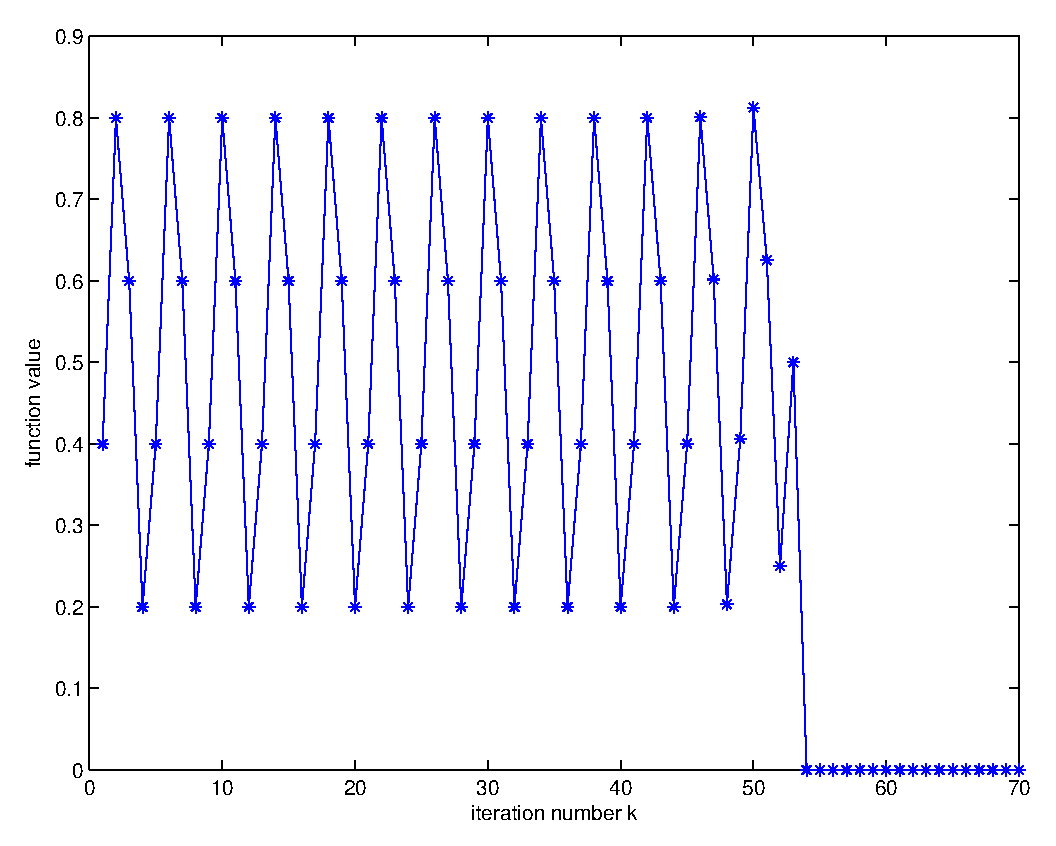
\includegraphics[width=0.4\textwidth]{doubling.eps}\\
  \caption{一个简单的例子, 表明舍入误差可能对一个算法造成很大的影响}
  \label{fig:doubling}
\end{figure}

实际上, 关于为什么不带最小二乘的几何构建算法算不好大规模的精确距离的问题 
(尽管理论上很完美),
这个例子也可以给我们一些洞见, 误差累积是这个迭代算法一个很重要的因素.
在带误差的情形中, 距离误差带来的定位的不精确比累积误差大得多,
这会对迭代计算产生更大的影响. 
从这里也可以看出为什么带大的距离噪音的距离几何问题如此困难.



%%%%%%%%%%%%%%%%%%%%%%%%%%%%%%%
%%% 附件部分
%%%%%%%%%%%%%%%%%%%%%%%%%%%%%%%
\backmatter
    
  % 参考文献
  % 使用 BibTeX
  \bibliographystyle{myplain}
  \bibliography{bib/ref}
  
  \newpage 
  \phantomsection 
  \cleardoublepage
  \printindex

  
\begin{publications}{99}

\item Zaikun Zhang, Sobolev Seminorm with Applications to Derivative-Free
    Optimization, 2011, submitted.
\item Zaikun Zhang, Notes on the Sobolev (Semi)Norms of Quadratic Functions
    2011, finished.
\item Zaikun Zhang, A Fast Derivative-Free Optimization Algorithm with Subspace
    Technique, 2012, finished.

\end{publications}

  % 个人简历
  
\begin{resume}
    张在坤,男,山东省临朐县大郝庄村人,1985 年 8 月生。
%    23 日\footnote{乙丑年七月初八。}生。

张在坤 2003 年 9 月至 2007 年 7 月就读于吉林大学数学学院信息与计算科学专业,获
学士学位;2007 年 9 月至 2012 年 7 月于中国计算数学与科学工程计算研究所
攻读博士学位,研究方向为最优化理论与应用。

Email:
\href{mailto:zaikunzhang@gmail.com}{\texttt{zaikunzhang@gmail.com}},
\href{mailto:zhangzk@lsec.cc.ac.cn}{\texttt{zhangzk@lsec.cc.ac.cn}}。
\end{resume}

  % 致谢
  
\begin{thanks}
博士论文写完了,二十一年的求学生活随之进入尾声。回首往事,我心中充满感激。
我有太多的人需要感谢。

首先,我要感谢我的导师、我最敬爱的袁老师。2006 年保研的时候,我其实并没有想
好要选择什么专业。六年前的那个下午,当我敲开袁老师的门,第一眼看到袁老师的
时候,就被老师的学者风度打动了。我依然清晰地记得那天袁老师与我面对面交谈的
情景,那是我第一次见到如此平易近人的老师。从那一刻起我就决定要做袁老师的学生。
如今,即将从袁老师这里毕业,我为当初的选择感到幸运。感谢袁老师五年来提供的宽松的研究
环境,让我可以研究自己喜欢的问题;感谢袁老师细心的指导,让我领略到优化之美,
领略到数学家思考问题的方式;感谢袁老师一直以来的鼓励和提携;感谢袁老师给我
出国访问的机会。我还要特别感谢袁老师在生活上对我的关心和照顾。五年里,袁老
师一直给予我父亲一般的关怀。2010 年夏天与袁老师在欧洲的三个月里,袁老师给我
做饭,带我旅游,让我懂得了什么叫师徒如父子。感谢袁老师一次又一次对我的教诲,
教给我生活的道理,分享给我人生的经验。是袁老师让我重新认识了生活。从袁老师
身上学到的每一点都是我最宝贵的财富。谢谢您,袁老师!

感谢我的师母张焱女士。感谢师母一直以来在生活上的关心和照顾。师母和袁老师让
我在北京感受到了家的温暖。我可能是被师母和袁老师叫到家里吃饭最多的学生。2010 
年夏天在欧洲的日子里,师母和袁老师像家人一样待我,让我度过了一段难忘的日子。
那段时间师母做的汤是世界上最好喝的汤。师母无论多忙,都会时常关心我的生活和
工作,让我心中多了一份前进的动力。

特别感谢袁老师的导师、英国皇家学会会员、美国科学院外籍院士、首届 Dantzig 奖
获得者、剑桥大学的 \mbox{M. J. D. Powell} 教授给我提供的指导和帮助。Powell 
教授对后辈的热情让我感动。每一次向 Powell 教授请教都让我获益匪浅。Powell 教
授提供了 \newuoa 算法的源代码和参考文献,这是我五年学习和研究中最重要的素材。

感谢德国拜罗伊特大学的 Klaus Schittkowski 教授和夫人。在 2010 年夏天我访问
拜罗伊特大学期间,教授和夫人给予了热情周到的接待,令我十分难忘。在拜罗伊特
的日子是这五年里我度过的最美好的时光。感谢洪堡基金资助我这次访问。本文
第\ref{chap:sobolev}章的部分内容就是在此次访问期间完成的。

感谢课题组的戴彧虹老师。戴老师在讨论班上的指点让我获益匪浅,这在论文里有直
接体现。戴老师豁达的生活态度和平易近人的风度永远值得我学习。感谢课题组的刘
歆老师。感谢刘老师五年以来像兄长一样的鼓励和帮助。

感谢课题组的夏勇博士、徐姿博士、牛凌峰博士、李在禾博士、付云姗博士、唐明筠
博士、程明厚博士、宫鲁津博士、郝春林博士、寇彩霞博士、费存林、
顾晓娟博士和李庆娜博士等师姐师兄们,感谢孙聪、张睿燕、姜波、Thanawath 
Niyamosoth、张文慧、刁瑞、刘田香、盛镇醴、崔春风、董乾和王树雄等师妹师弟和
同学们。感谢我的师兄丁晓东博士。我接触无导数优化算法就是从听师兄的报告开始的;
师兄在我研究的起步阶段提供了很多帮助,我使用的很多参考文献都是师兄提供的。
感谢与我同一级的王晓、刘亚锋和吴乐秦,和他们一起度过的五年,点点滴滴都值得
回忆。

Powell 教授、葡萄牙 Universidade de Coimbra 的 Lu\'{i}s Nunes Vicente 教授、
美国 Louisiana State University 的张洪超博士 (我的师兄) 以及李庆娜师姐、孙
聪师妹和姜波师弟审阅了我的第一篇论文 \cite{SobolevDFO} 并提出了宝贵的意见。
感谢他们对我的无私帮助。

感谢我在北京期间的室友张乔夫和张新雨、翟建梁两位师兄。我经常早出晚归,影响
了他们休息,感谢他们对我的包容。

感谢与我一同入所的何连花、梁珊、孙建青、王满、陈冲、陈耀、成杰、戴银云、黄
记祖、马云飞、伍泽东、肖俊敏和张乔夫。五年与他们一起走过我很荣幸。


感谢吴继萍老师、白英老师、丁如娟老师、樊建荣老师、刘颖老师、钱莹老师、张纪
平老师、魏敏老师、关华老师、王璐璐老师、邵欣老师和尹永华老师五年期间对我的
帮助。

感谢我的母校、我深怀眷恋的吉林大学。人生最美好的四年能在吉大度过,我很幸运。
特别感谢吉林大学数学学院的老师们。感谢谢敬然老师。谢老师并不认识我,但是是
他的引导让我走入了数学的美妙世界。感谢马富明老师。马老师对学生的爱护和提携
是我学习的榜样。感谢李永海老师。李老师对学生的真诚让人感动。感谢纪友清老师。
纪老师讲授的泛函分析塑造了我的思维方式。感谢大学四年所有教过我的老师。从他
们身上,我学到了很多很多。

特别感谢我的启蒙老师夏翠苓女士。回首漫漫求学路,我取得的每一点进步都深深地
植根于您二十年前的教诲。

感谢中学和大学里与我一起笑过、哭过、奋斗过的兄弟们。有你们在,我活得很踏实。
特别感谢王振宇、张明涛、石胜坤和张旭升。五年里,你们一直是我在北京最可靠的
后盾。

最后,我要感谢我的家人。感谢我深爱的父亲母亲。做你们的儿子是我此生最幸运的
事情;是你们教会我,诚实的劳动是获得成功的唯一方法;在我 失落的时候,你们是
我内心最大的慰藉;在我遭受挫折的时候,想到你们我总能找回前进的勇气。谢谢你
们,我爱你们!感谢我的哥哥和嫂子,感谢他们一直以来对我的照顾。若没有哥哥当
初的建议,我不会报考吉林大学数学学院,这是改变我一生的事情。

本文完成之后的第十天 (壬辰年三月廿七) 是母亲六十岁生日。
我谨以此文作为献给母亲的生日礼物,祝母亲健康、平安。

%\begin{flushright}
%    {\kaishu{张在坤}}\\
%    2012 年 4 月 7 日\\
%    于北京保福寺
%\end{flushright}
\begin{flushright}
    {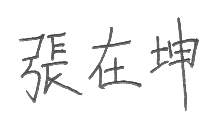
\includegraphics[width=0.16\textwidth]{zzk.eps}}\\
    2012 年 4 月 7 日\\
    于北京保福寺
\end{flushright}
\end{thanks}


\end{document}


